\documentclass[12pt,letterpaper]{article}

\usepackage{amsmath, amsthm}
\usepackage{microtype, parskip}
\usepackage[comma,numbers,sort&compress]{natbib}
\usepackage{lineno}
\usepackage{docmute}
\usepackage{caption, subcaption, multirow, morefloats, rotating}
\usepackage{wrapfig}

\frenchspacing

\begin{document}

\section*{Results}

The results of the anlyses described above take one of two forms: direct inspection of parameter posterior estimates from both models, and downstream estimates of diversity and diversification rates based on posterior predictive simulations from the birth-death model; the reason for which is explained below in the comparison of the models' posterior predictive check results.

\subsection*{Comparing parameter estimates from the pure-presence and birth-death models}

% look at the posterior predictive checks
%   which model has better fit
%   what does that mean?


\begin{figure}[ht]
  \begin{subfigure}[b]{0.45\textwidth}
    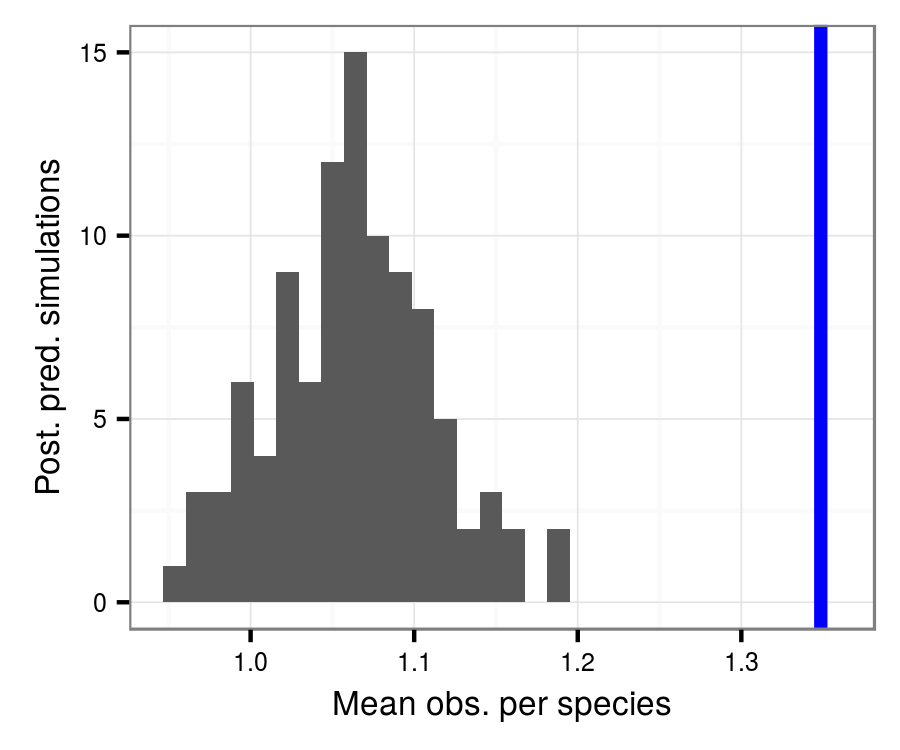
\includegraphics[width=\textwidth,height=0.4\textheight,keepaspectratio=true]{figure/pred_occ}
    \caption{Pure-presence model}
    \label{fig:ppc_pure_presence}
  \end{subfigure}
  \begin{subfigure}[b]{0.45\textwidth}
    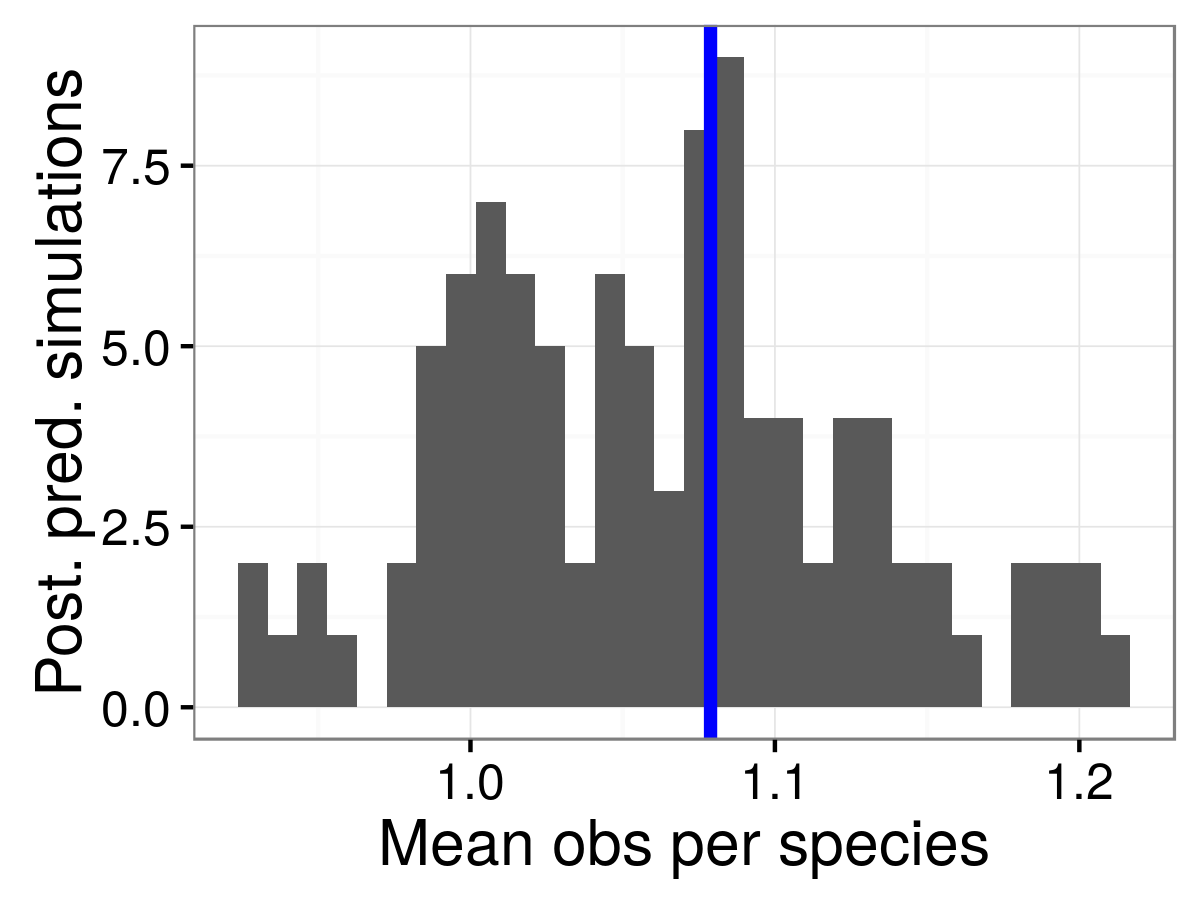
\includegraphics[width=\textwidth,height=0.4\textheight,keepaspectratio=true]{figure/pred_occ_bd}
    \caption{Birth-death model}
    \label{fig:ppc_birth_death}
  \end{subfigure}
  \caption[Posterior predictive check of average occurrence]{Comparison of the average observed number of occurrences per species (blue line) to the average number of occurrences from 100 posterior predictive datasets using the posterior estimates from the pure-presence and birth-death models.}
  \label{fig:ppc}
\end{figure}

Comparison of the posterior predictive results from the pure-presence and birth-death models reveals a striking difference in performance of either model to preidct the structure of the underlying data (Fig. \ref{fig:ppc}). The simulated datasets generated from the birth-death model are clearly able to better reproduce the observed average number of occurrence than the pure-birth model which greatly underestimates the ovserved average number of occurrences. This result means that inferences based on the birth-death model are more likely to be representative of the underlying data than inferences based on the pure-presence model. Further inspection of the posterior parameter estimates from both models gives further insight into the resons for this difference in posterior predictive results \citep{Gelman2013d}. 


Occurrence probabilities estimated from the pure-presence model (Fig. \ref{fig:eco_occur}) are broadly similar to the estimates of origination probability from the birth-death model (Fig. \ref{fig:eco_origin}) but not the survival probability estimates (Fig. \ref{fig:eco_survival}). This result supports the idea that changes to the North American regional species pool is more likely due to changes in origination than extinction, a result that is returned to later in the discussion of per-capita diversification, origination, and extinction rates.

For most ecotypes, both estimated occurrence probabilities from the pure-presence model (Fig. \ref{fig:eco_occur}) and origination probabilities estimated from the birth-death model (Fig. \ref{fig:eco_origin}) increase with time. This makes sense given that, over time, all species that have at least one observed occurrence must have had that occurrence by the last time point, so our certainty in a species occurring must increase with time. Importantly, there are potential issues surrounding the partial identifiability of the observation parameters \(p\) which may contribute to edge effects in estimates of occurrence, origination, and extinction \citep{Royle2008}. Notably, ecotypes with arboreal components do not appear to follow a similar pattern; instead, occurrence and origination probabilities appear relatively flat for most of the Cenozoic; this is most likely caused by those species of those ecotypes no longer originating or originating very rarely.

The dramatic differences in the estimates origination and survival probabilities are indicative of how differently these processes affect the diversification process and may also be responsible for the better posterior predictive perfomance of the birth-death model over the pure-presence model (Fig. \ref{fig:ppc_pure_presence}, and \ref{fig:ppc_birth_death}). While the estimates at all points along both time series have high variance, what is striking is how mean origination probability changes over time while most ecotype survival probabilities have relatively stable means for the entire Cenozoic (Fig. \ref{fig:eco_origin}, and \ref{fig:eco_survival}).

For most ecotypes, the estimates of origination probabilities are with less uncertainty than similar estimates of survival probabilities (Fig. \ref{fig:eco_origin}, and \ref{fig:eco_survival}). In logistic regression, high uncertainty in the estimates of the underlying log-odds of occurrence, origination, or survival tends to be indicative of extreme rarity or complete absence of the specific ecotype; the latter is called complete separation which occurs when there is no uncertainty in the effect of a covariate on presence/absence, the effect of which has been mitigated by the hierarchical modeling strategy used here \citep{Gelman2013d,Gelman2007} CITATION Statistical Rethinking.


\begin{figure}[ht]
  \centering
  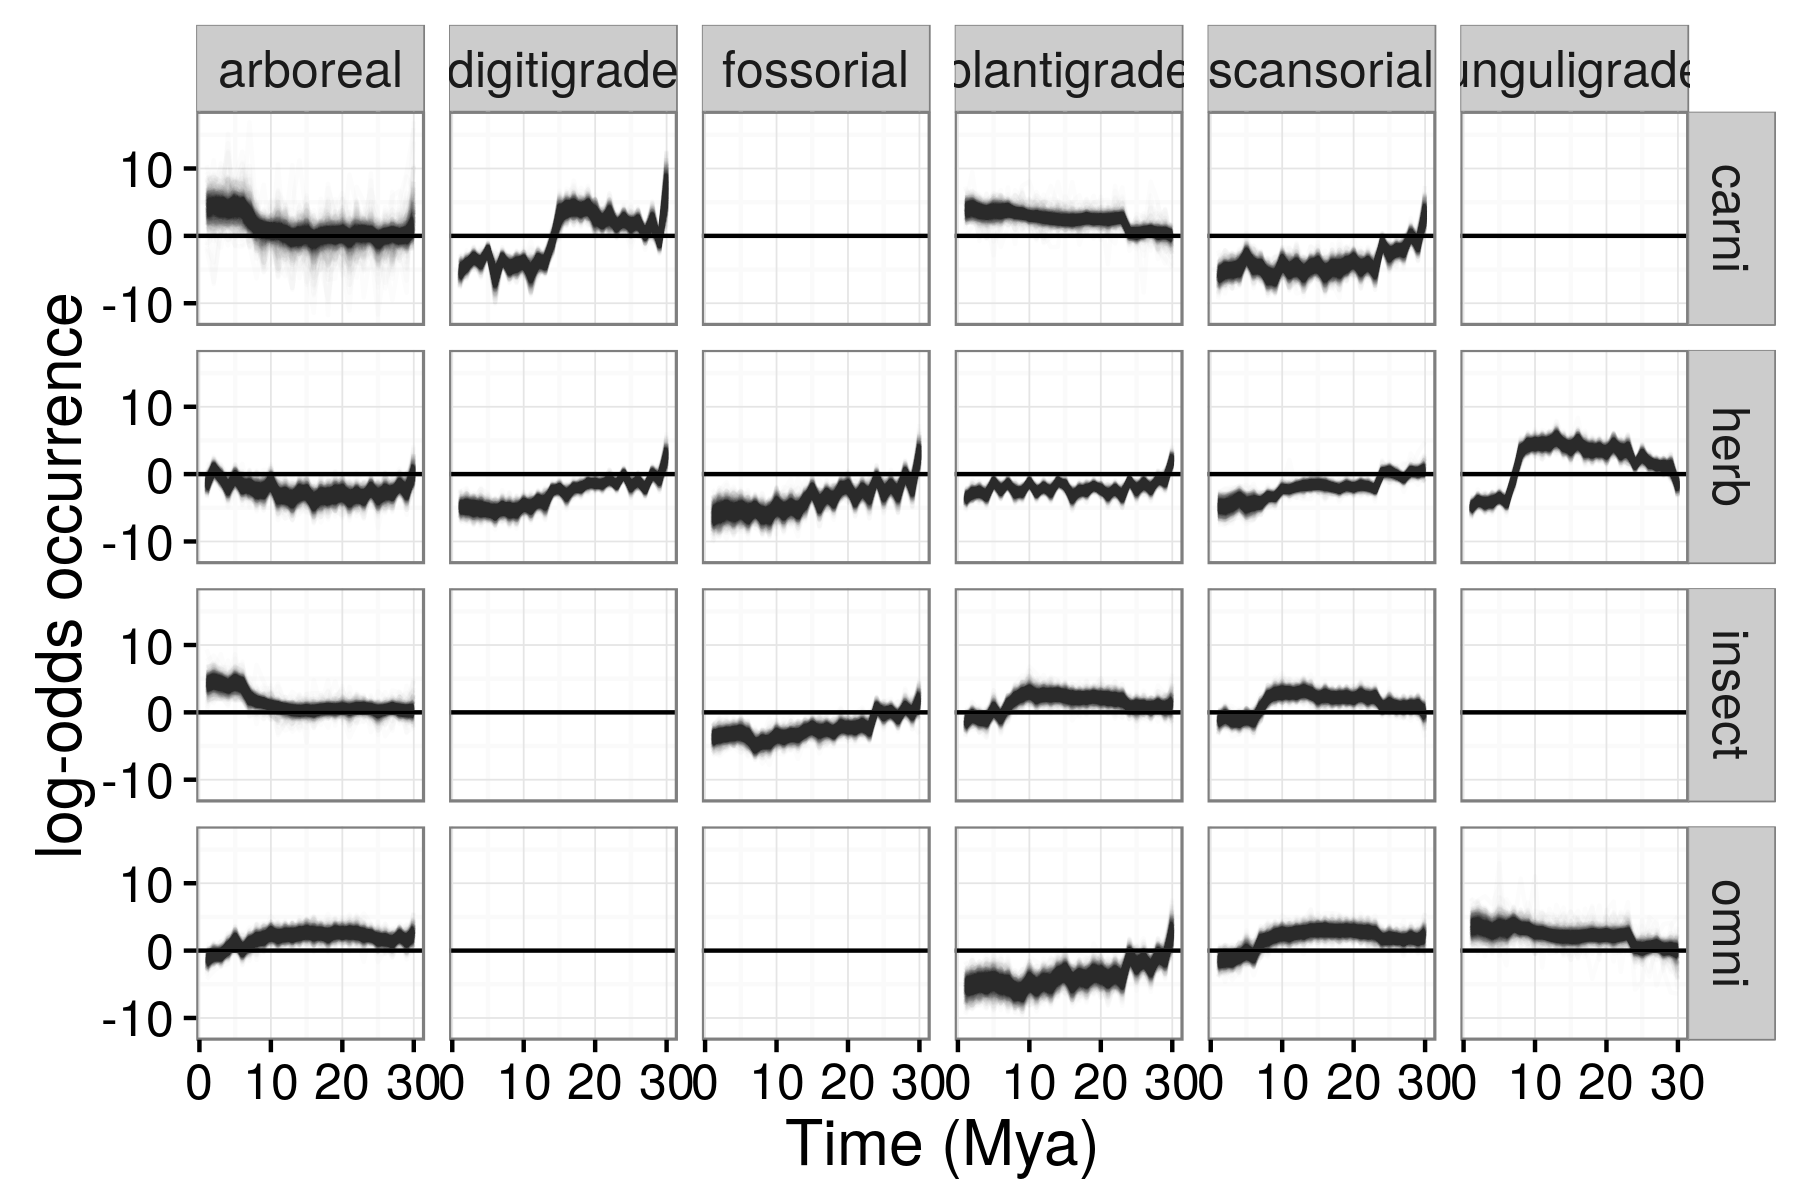
\includegraphics[width=\textwidth,height=0.4\textheight,keepaspectratio=true]{figure/ecotype_occurrence}
  \caption[Ecotype occurrence probability estimated from the pure-presence model]{Probability of a mammal ecotype occurring over time as estimated from the pure-presence model. Each panel depicts 100 random samples from the model's posterior. The columns are by locomotor category and rows by dietary category; their intersections are the observed and analyzed ecotypes. Panels with no lines are ecotypes not observed in the dataset.}
  \label{fig:eco_occur}
\end{figure}

\begin{figure}[ht]
  \centering
  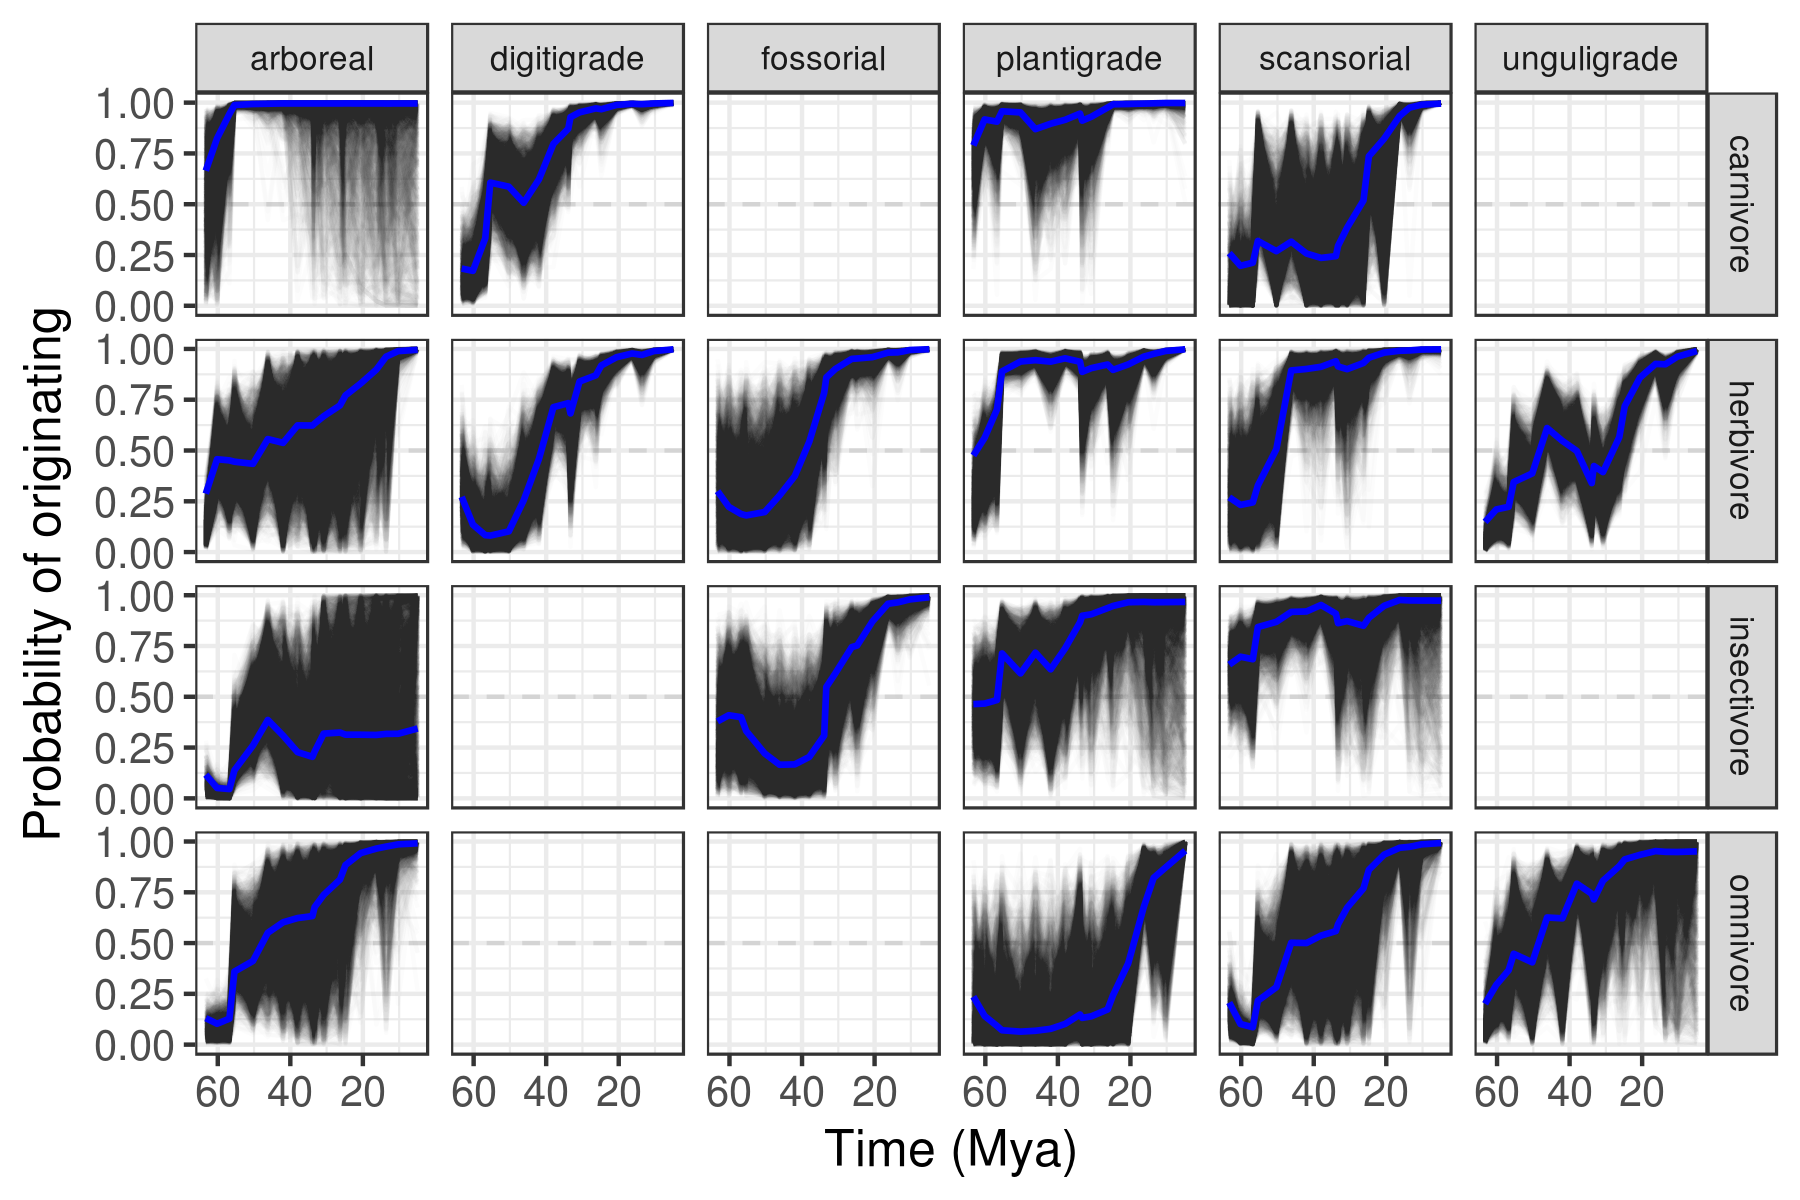
\includegraphics[width=\textwidth,height=0.4\textheight,keepaspectratio=true]{figure/ecotype_origin_bd}
  \caption[Ecotype origination probability estimated from the birth-death model]{Probability of a mammal ecotype origination probabliities at each time point as estimated from the birth-death model. Each panel depicts 100 random samples from the model's posterior. The columns are by locomotor category and rows by dietary category; their intersections are the observed and analyzed ecotypes. Panels with no lines are ecotypes not observed in the dataset.}
  \label{fig:eco_origin}
\end{figure}

\begin{figure}[ht]
  \centering
  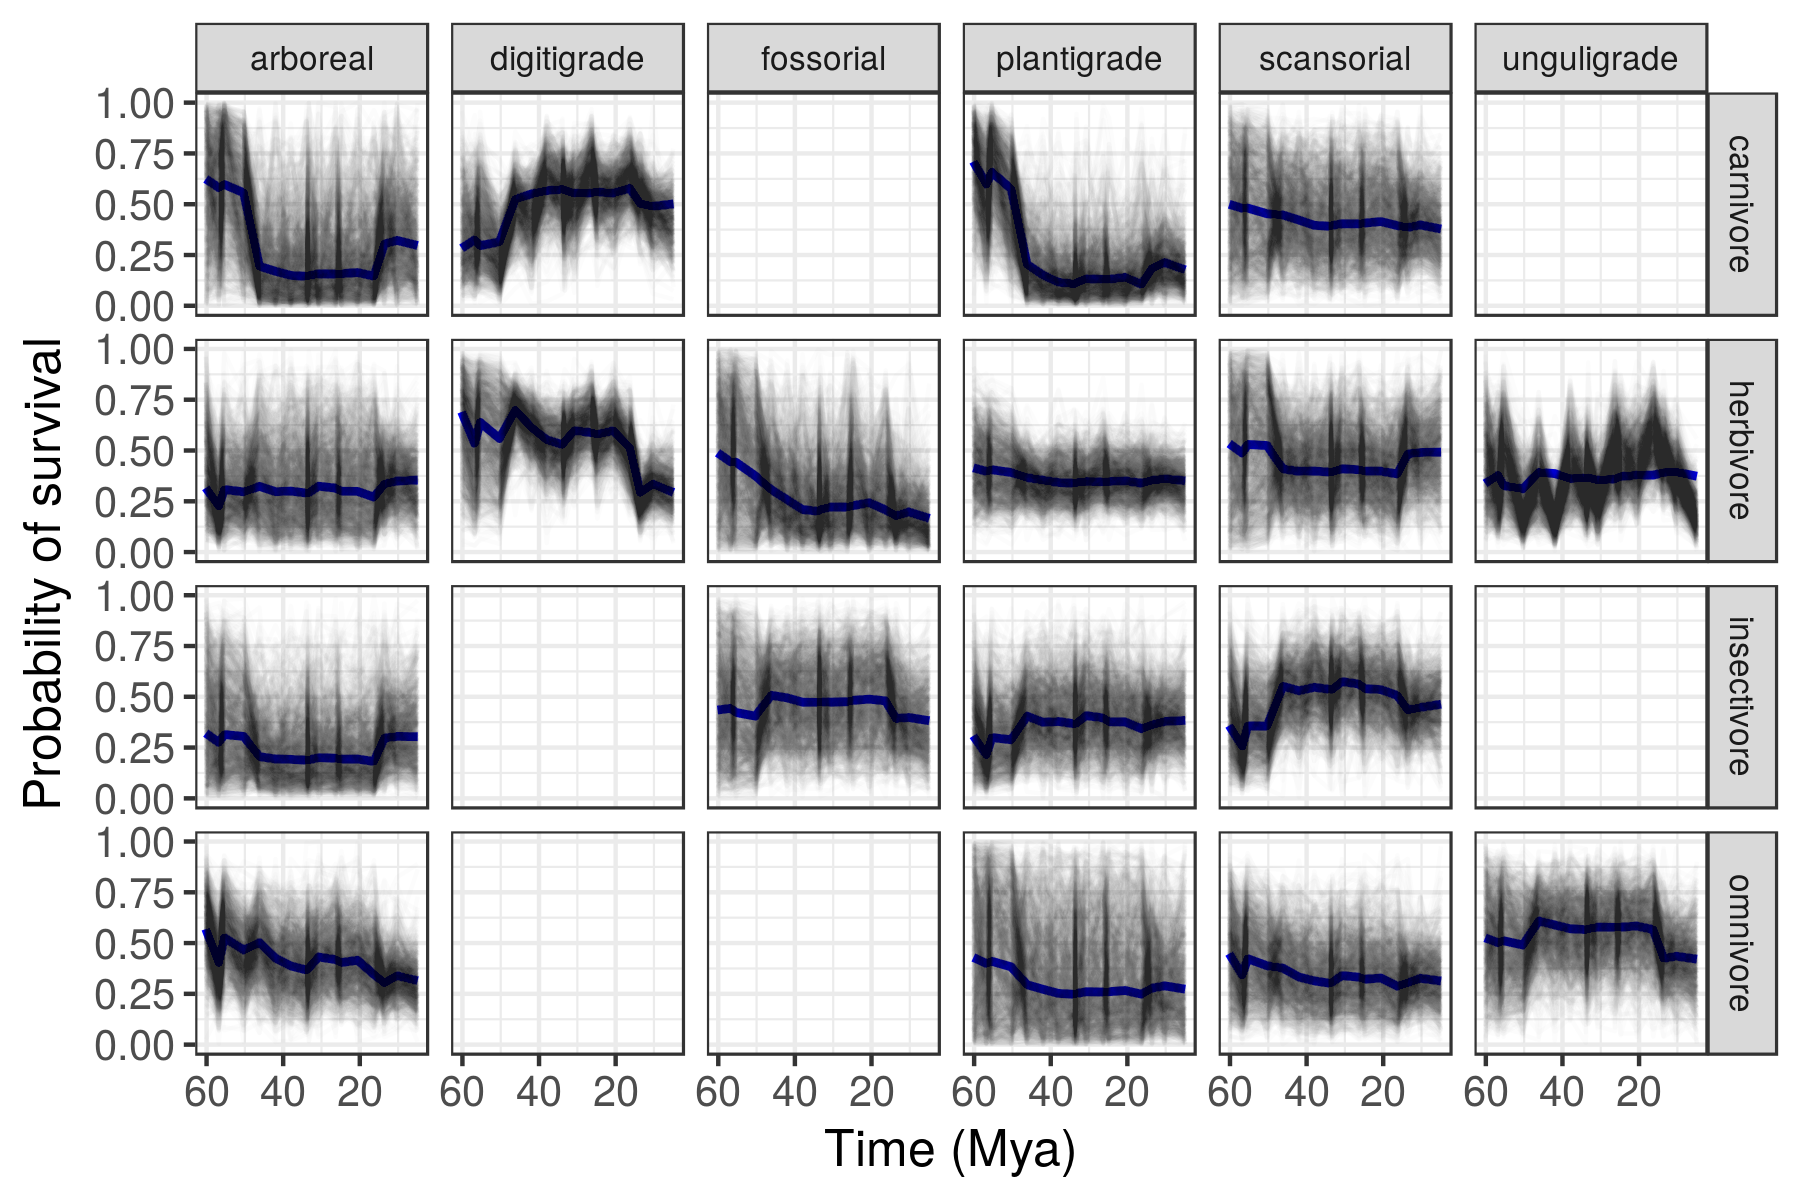
\includegraphics[width=\textwidth,height=0.4\textheight,keepaspectratio=true]{figure/ecotype_survival_bd}
  \caption[Ecotype survival probability estimated from the birth-death model]{Probability of a mammal ecotype survival probabilities at each time point as estimated from the birth-death model. Each panel depicts 100 random samples from the model's posterior. The columns are by locomotor category and rows by dietary category; their intersections are the observed and analyzed ecotypes. Panels with no lines are ecotypes not observed in the dataset.}
  \label{fig:eco_survival}
\end{figure}





The pure-presence and birth-death models also differ in the estimated effect of mass on the probability of sampling a species that is present (Fig. \ref{fig:mass_preserve}). For the pure-presence model, mass is estimated to not have a strong effect on the probability of sampling a species that is presence (Fig. \ref{fig:mass_preserve_pure_pres}). Contrastingly, for the birth-death model mass is found to have a negative relationship with observation such that larger species are less likely to be observed if present than smaller species (Fig. \ref{fig:mass_preserve_bd}). 

The result from the birth-death model may be considered unexpected given that it is generally assumed that larger mammals are more likely to have been collected than smaller mammals CITATION. However, collection is not preservation; similarities in preservation rate indicate similarities in how gap-filled species records are. What this result means is that the record of large bodied species is expected on average to have more gaps in sampling and a less consistent record from time point to time point than smaller bodied species. Additionally, as this is presence/absence data higher preservation and collection in terms of individual specimens at a location or a single temporal horizon does not necessarily translate to high preservation over multiple time points.

The average sampling probabilities for both the pure-presence model and birth-death model are both at the point where (rescaled log) mass equals 0; visual comparison indicates that, on average, sampling probability has greater posterior estimate in the pure-presence model than the birth-death model (Fig.\ref{fig:mass_preserve}). The probability that one estimate is different from the other, however, are not directly calculable as they come from different models; what this tells us is how adding more information to the model (i.e. replacing occurrence with origination and extinction) changes parameter estimates in the model.

\begin{figure}[ht]
  \begin{subfigure}[b]{0.45\textwidth}
    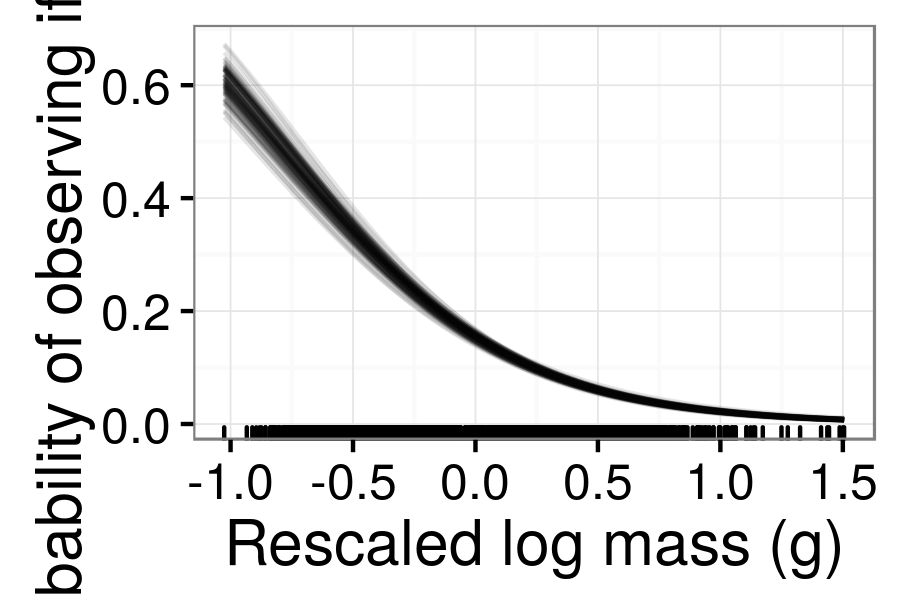
\includegraphics[width=\textwidth,height=0.4\textheight,keepaspectratio=true]{figure/mass_on_samp}
    \caption{Pure-presence model}
    \label{fig:mass_preserve_pure_pres}
  \end{subfigure}
  \begin{subfigure}[b]{0.45\textwidth}
    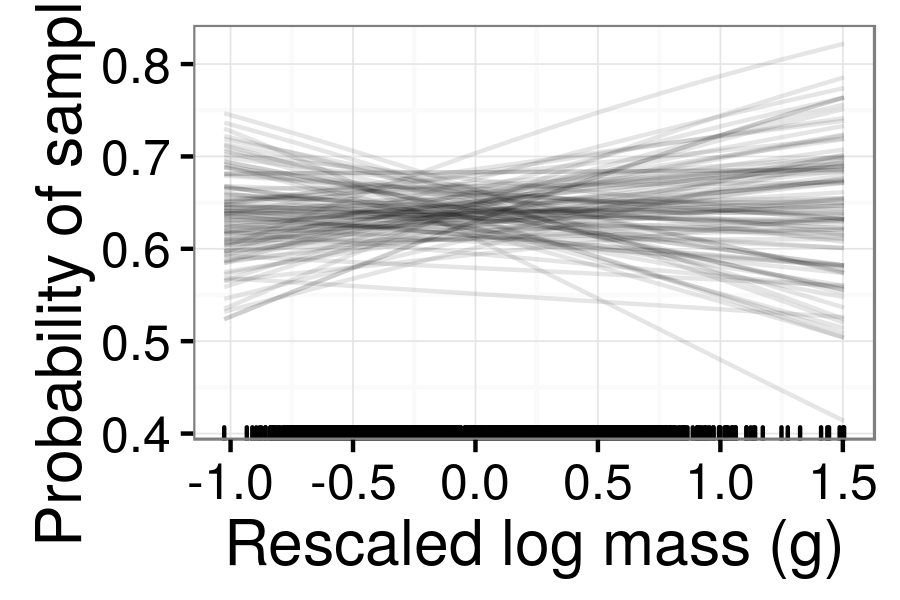
\includegraphics[width=\textwidth,height=0.4\textheight,keepaspectratio=true]{figure/mass_on_samp_bd}
    \caption{Birth-death model}
    \label{fig:mass_preserve_bd}
  \end{subfigure}
  \caption[Estimates of the effect of mass on observation probability]{Estimates of the effect of species mass on probability of sampling a present species (\(p\)). Mass has been log-transformed, centered, and rescaled; this means that a mass of 0 corresponds to the mean of log-mass of all observed species and that mass is in standard deviation units. Estimates are from both the pure-presence and birth-death models.}
  \label{fig:mass_preserve}
\end{figure}


The effect of species mass on probability of occurrence as estimated from the pure-presence (Fig. \ref{fig:mass_occur}) are most similar to the estimated effect of species mass on probability of origination for the birth-death model (Fig. \ref{fig:mass_origin}). The striking pattern observable in both sets of estimates is the higher probability of occurrence for species with body sizes closer to the mean than either extremes. This result is consistent with the canonically normal distribution of mammal body sizes \citep{Smith2004}; it is then expected that the most likely to occur species would be those from the middle of the distribution, and that species originating will on average be of average mass, especially considering species shared common ancestry \citep{Felsenstein1985b}. Note that all variation in estimates between ecotypes (Fig. \ref{fig:mass_origin}) is due to differences in ecotype-specific survival probability and the associated effects of plant phase; the effect of mass was considered constant for all ecotypes.

\begin{figure}[ht]
  \centering
  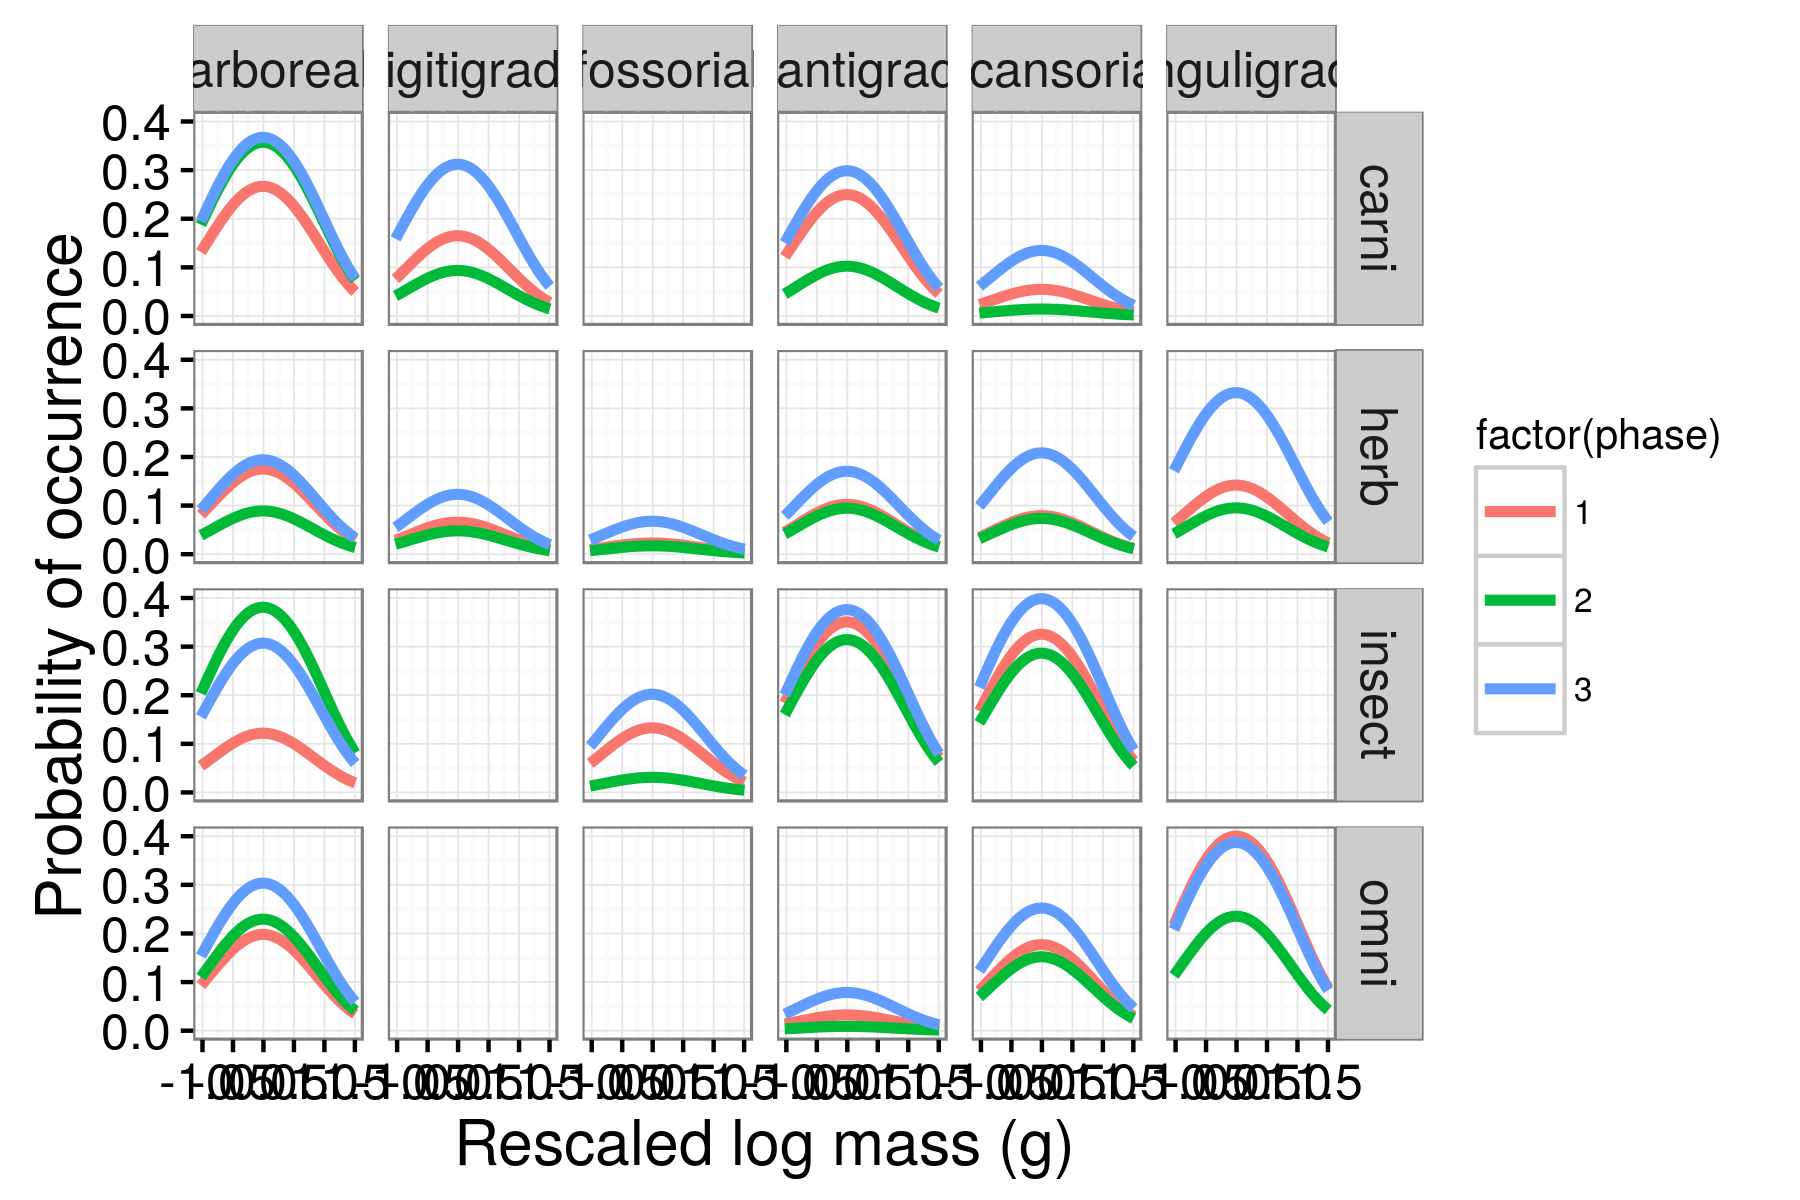
\includegraphics[width=\textwidth,height=0.4\textheight,keepaspectratio=true]{figure/mass_on_pres}
  \caption[Effect of mass on probability of species occurrence as estimated from the pure-presence model]{Mean estimate of the effect of species mass on the probability of a species occurrence for each of the three plant phases. The effect of mass is considered constant over time and that the only aspect of the model that changes with plant phase is the intercept of the relationship between mass and occurrence. The three plant phases are indicated by the color of the line. Mass has been log-transformed, centered, and rescaled; this means that a mass of 0 corresponds to the mean of log-mass of all observed species and that mass is in standard deviation units. Only the mean estimates of the effects of both mass and plant phase are plotted for clarity; these estimates are obviously made with uncertainty.}
  \label{fig:mass_occur}
\end{figure}

\begin{figure}[ht]
  \centering
  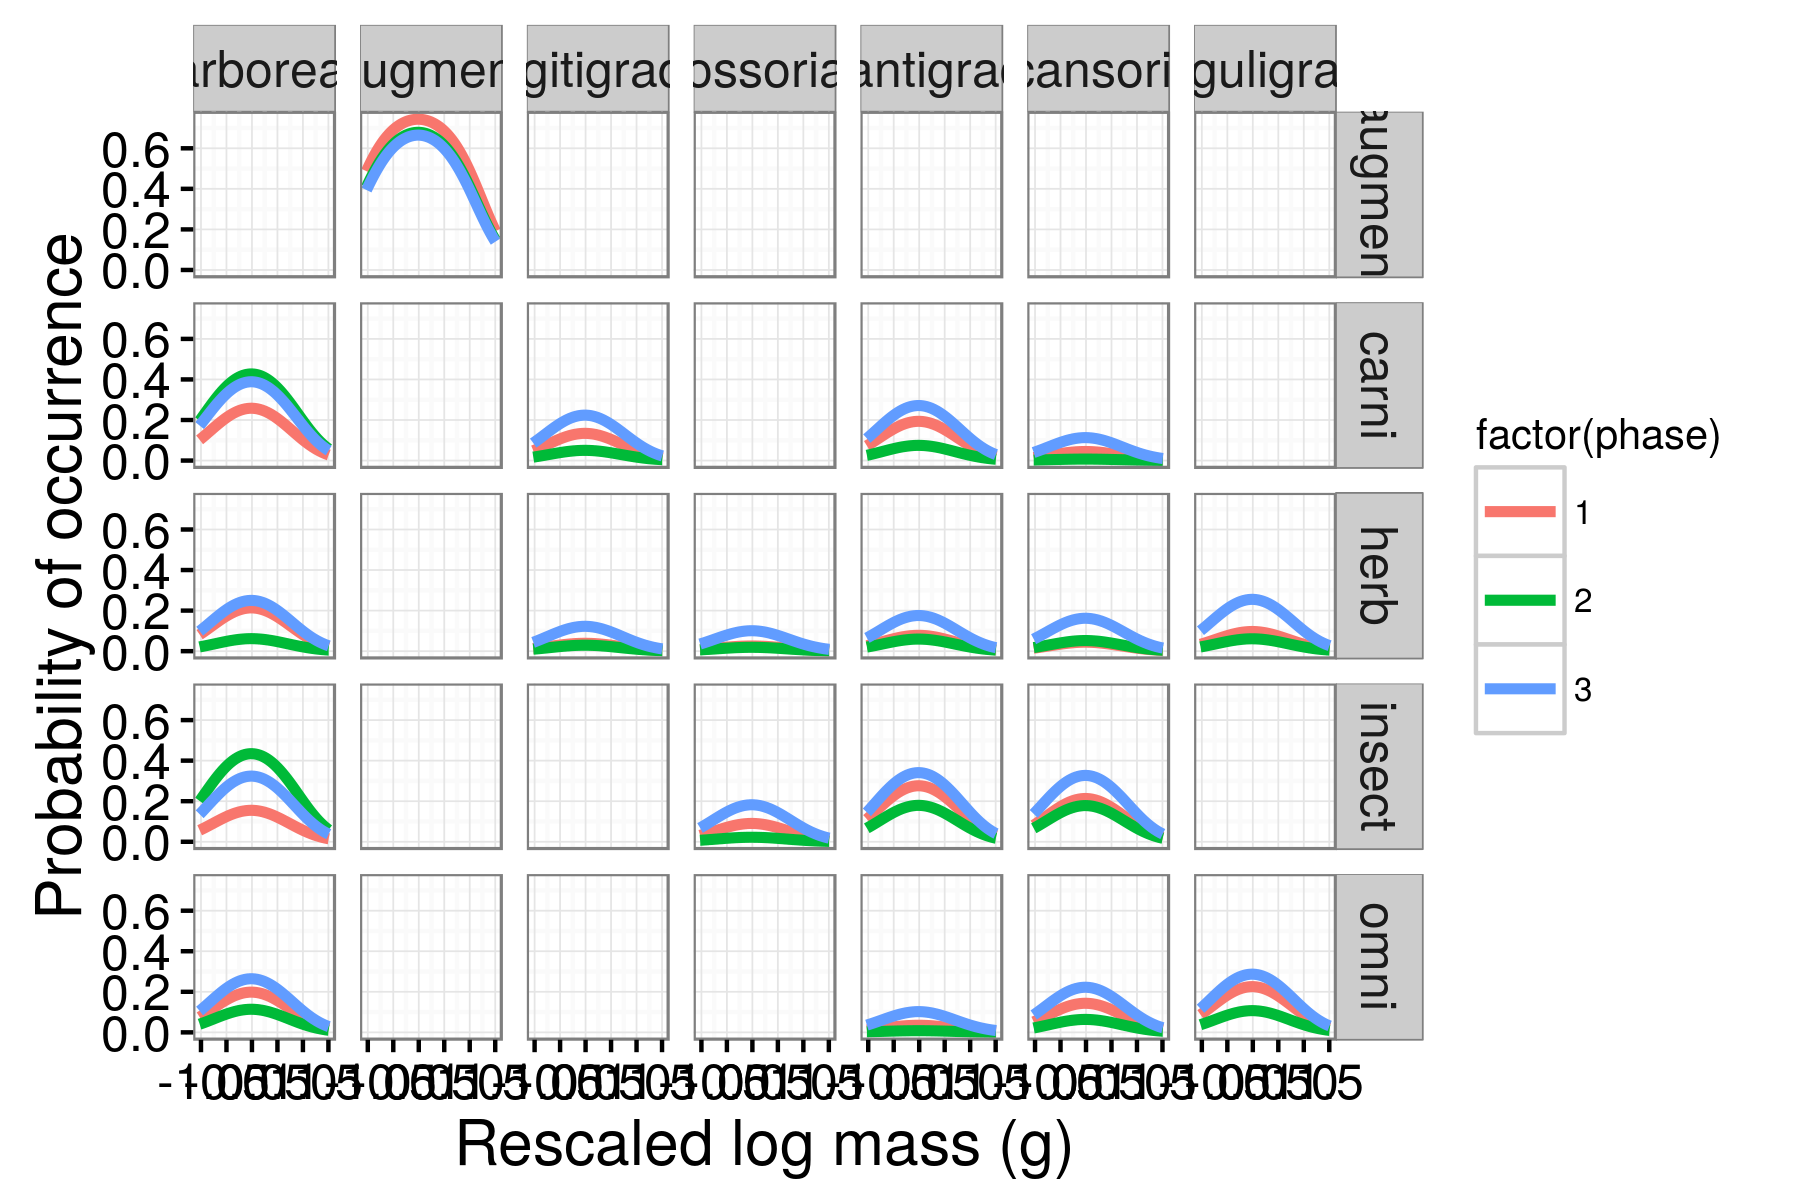
\includegraphics[width=\textwidth,height=0.4\textheight,keepaspectratio=true]{figure/mass_on_origin_bd}
  \caption[Effect of mass on probability of species origination as estimated from the birth-death model]{Mean estimate of the effect of species mass on the probability of a species originating for each of the three plant phases. The effect of mass is considered constant over time and that the only aspect of the model that changes with plant phase is the intercept of the relationship between mass and origination. The three plant phases are indicated by the color of the line. Mass has been log-transformed, centered, and rescaled; this means that a mass of 0 corresponds to the mean of log-mass of all observed species and that mass is in standard deviation units. Only the mean estimates of the effects of both mass and plant phase are plotted for clarity; these estimates are obviously made with uncertainty.}
  \label{fig:mass_origin}
\end{figure}



In contrast, the effect of species mass on probability of survival as estimated from the birth-death model (Fig. \ref{fig:mass_survival}) is consistent with previous findings that there is little effect of mass on extinction for North American mammals for the Cenozoic \citep{Smits2015b,Tomiya2013}. Note that all variation between ecotypes depicted in Figure \ref{fig:mass_survival} is due to differences in ecotype-specific survival probability and the associated effects of plant phase; the effect of mass was considered constant for all ecotypes (Eqs. \ref{eq:pure_presence}, \ref{eq:birth_death}).

\begin{figure}[ht]
  \centering
  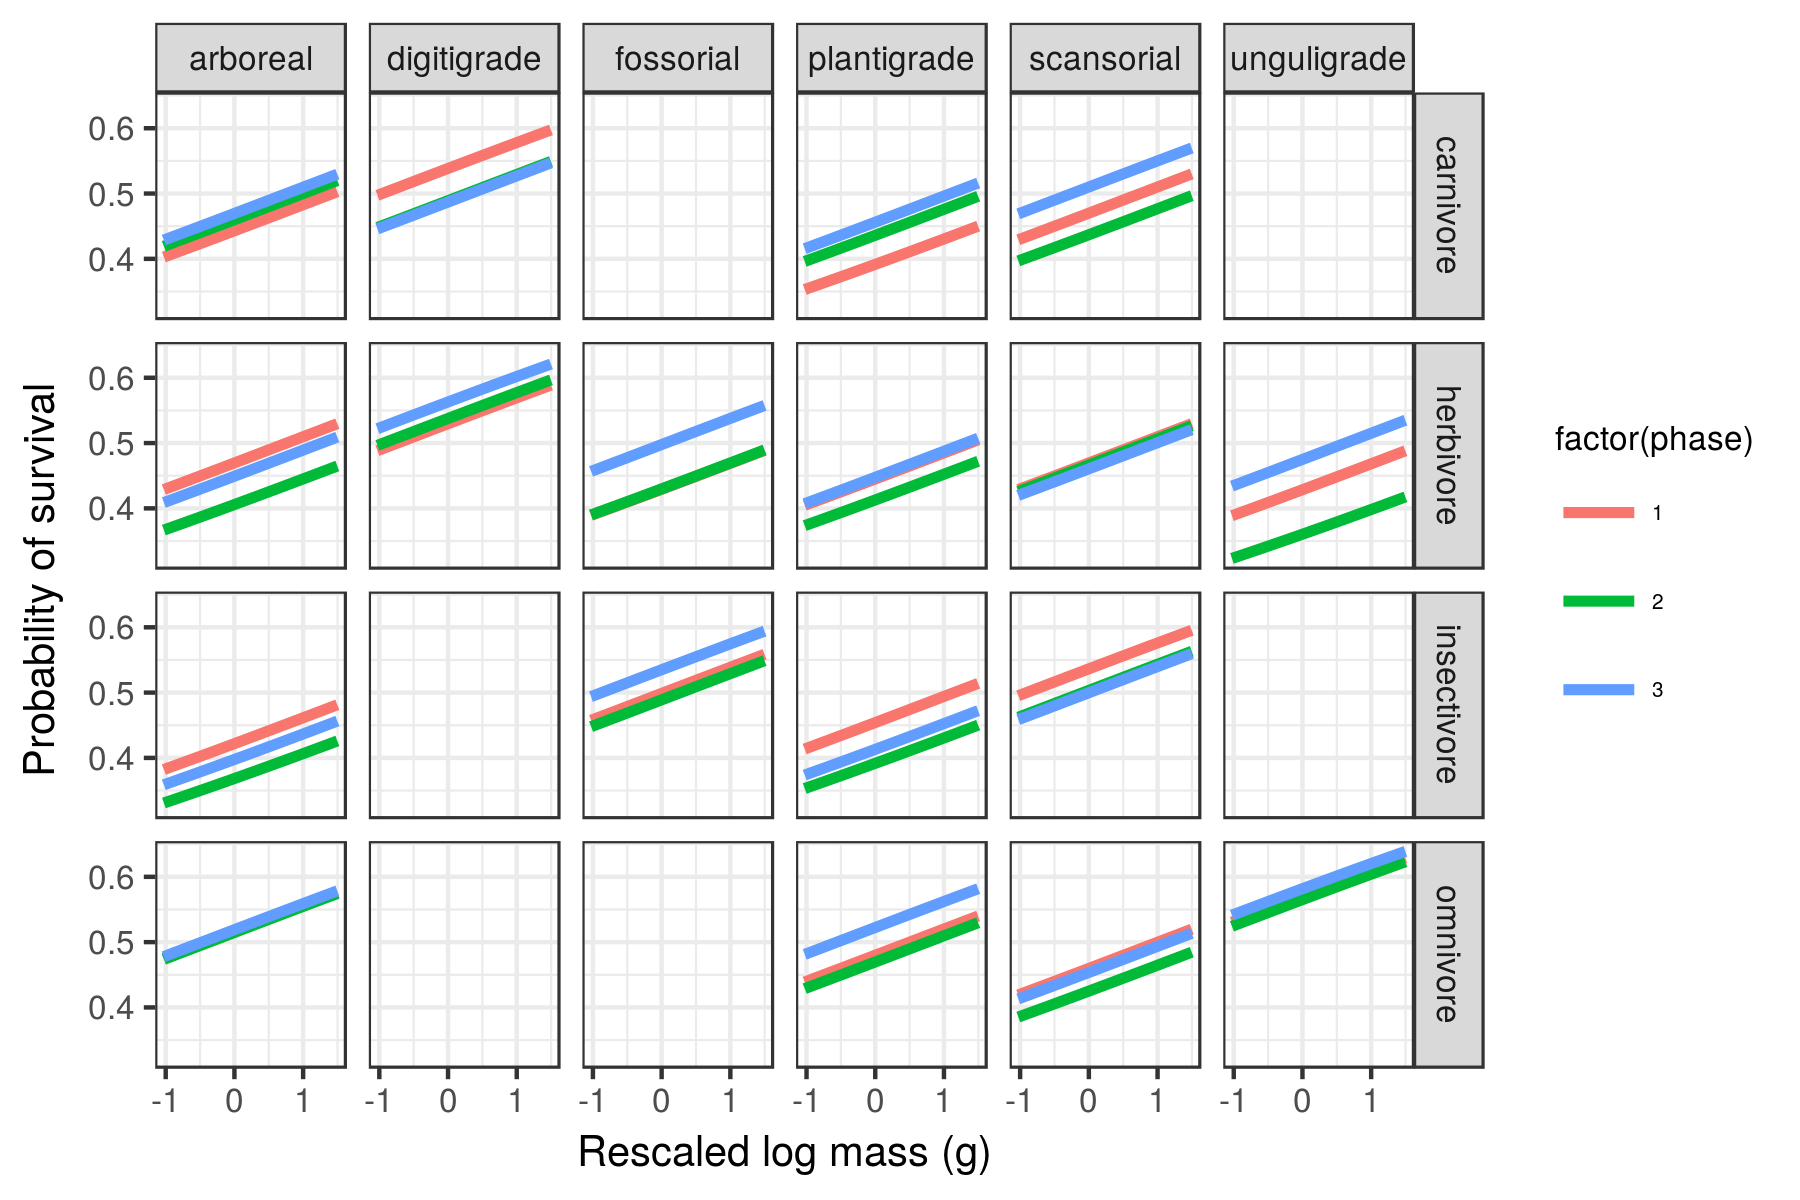
\includegraphics[width=\textwidth,height=0.4\textheight,keepaspectratio=true]{figure/mass_on_surv_bd}
  \caption[Effect of mass on probability of species survival as estimated from the birth-death model]{Mean estimate of the effect of species mass on the probability of a species survival for each of the three plant phases. The effect of mass is considered constant over time and that the only aspect of the model that changes with plant phase is the intercept of the relationship between mass and survival. The three plant phases are indicated by the color of the line. Mass has been log-transformed, centered, and rescaled; this means that a mass of 0 corresponds to the mean of log-mass of all observed species and that mass is in standard deviation units. Only the mean estimates of the effects of both mass and plant plant are plotted for clarity; these estimates are obviously made with uncertainty.}
  \label{fig:mass_survival}
\end{figure}



Similarities in parameters estimates between ecotypes may be due to similar response to environmental factors (Fig. \ref{fig:group_pure_presence}, \ref{fig:group_origin_bd}, and \ref{fig:group_surv_bd}). As with previous comparisons between posterior estimates from the pure-presence and birth-death models, the effects of the group-level covariates in the pure-presence model (Fig. \ref{fig:group_pure_presence})  are more similar to those estimates of the group-level effects on origination (Fig. \ref{fig:group_origin_bd}) as opposed to survival (Fig. \ref{fig:group_surv_bd}). As demonstrated in the comparisons of the effect of mass on occurrence from the pure-presence model (Fig. \ref{fig:mass_occur}) with the effect of mass on origination and survival from the birth-death model (Fig. \ref{fig:mass_origin}, and \ref{fig:mass_survival}), there is considerable variation in the effect of plant phases on ecotype-specific estimates.

  
\begin{figure}[ht]
  \centering
  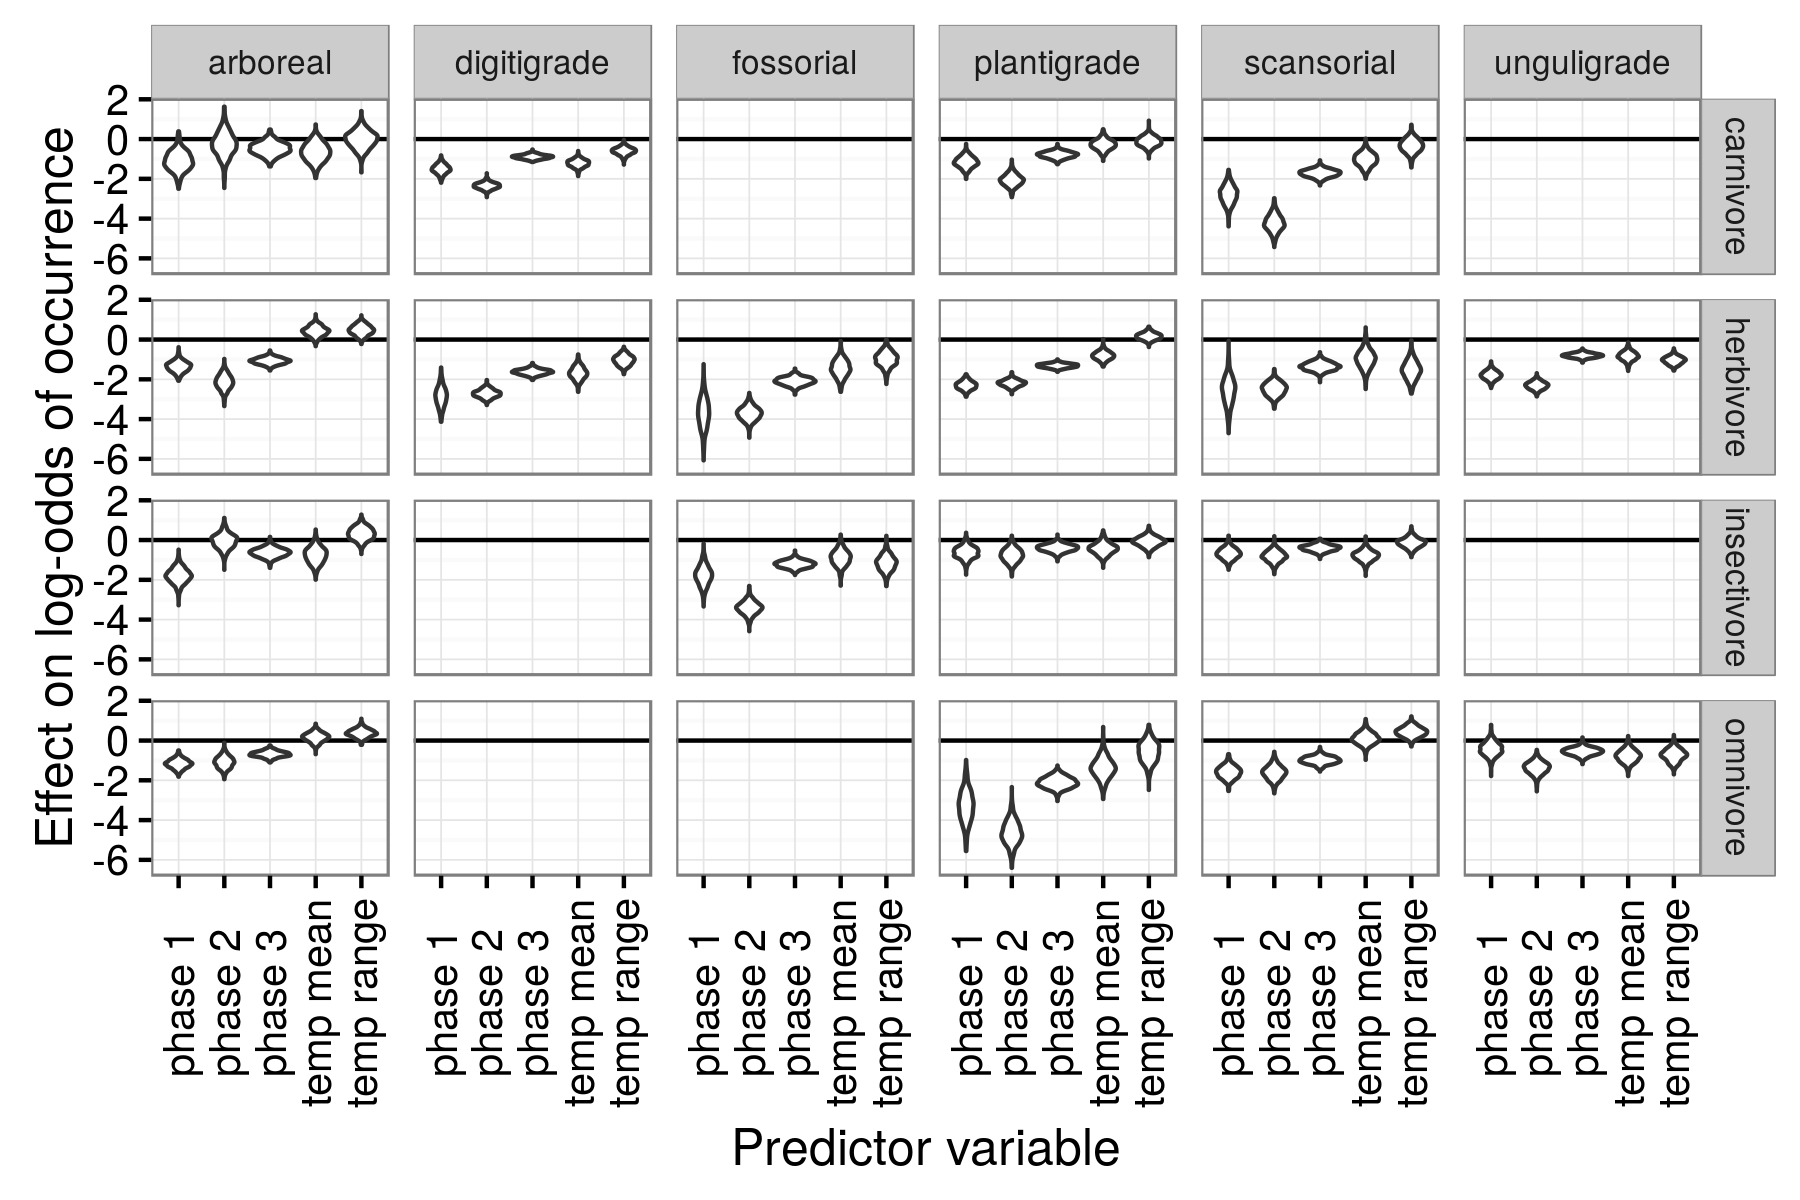
\includegraphics[width=\textwidth,height=0.4\textheight,keepaspectratio=true]{figure/group_on_ecotype}
  \caption[Effects of group-level covariates on log-odds of ecotype occurrence as estimated from the the pure-presence model]{Estimated effects of the group-level covariates describing environmental context on log-odds of species occurrence. These estimates are from the pure-presence model.} 
  \label{fig:group_pure_presence}
\end{figure}

\begin{figure}[ht]
  \centering
  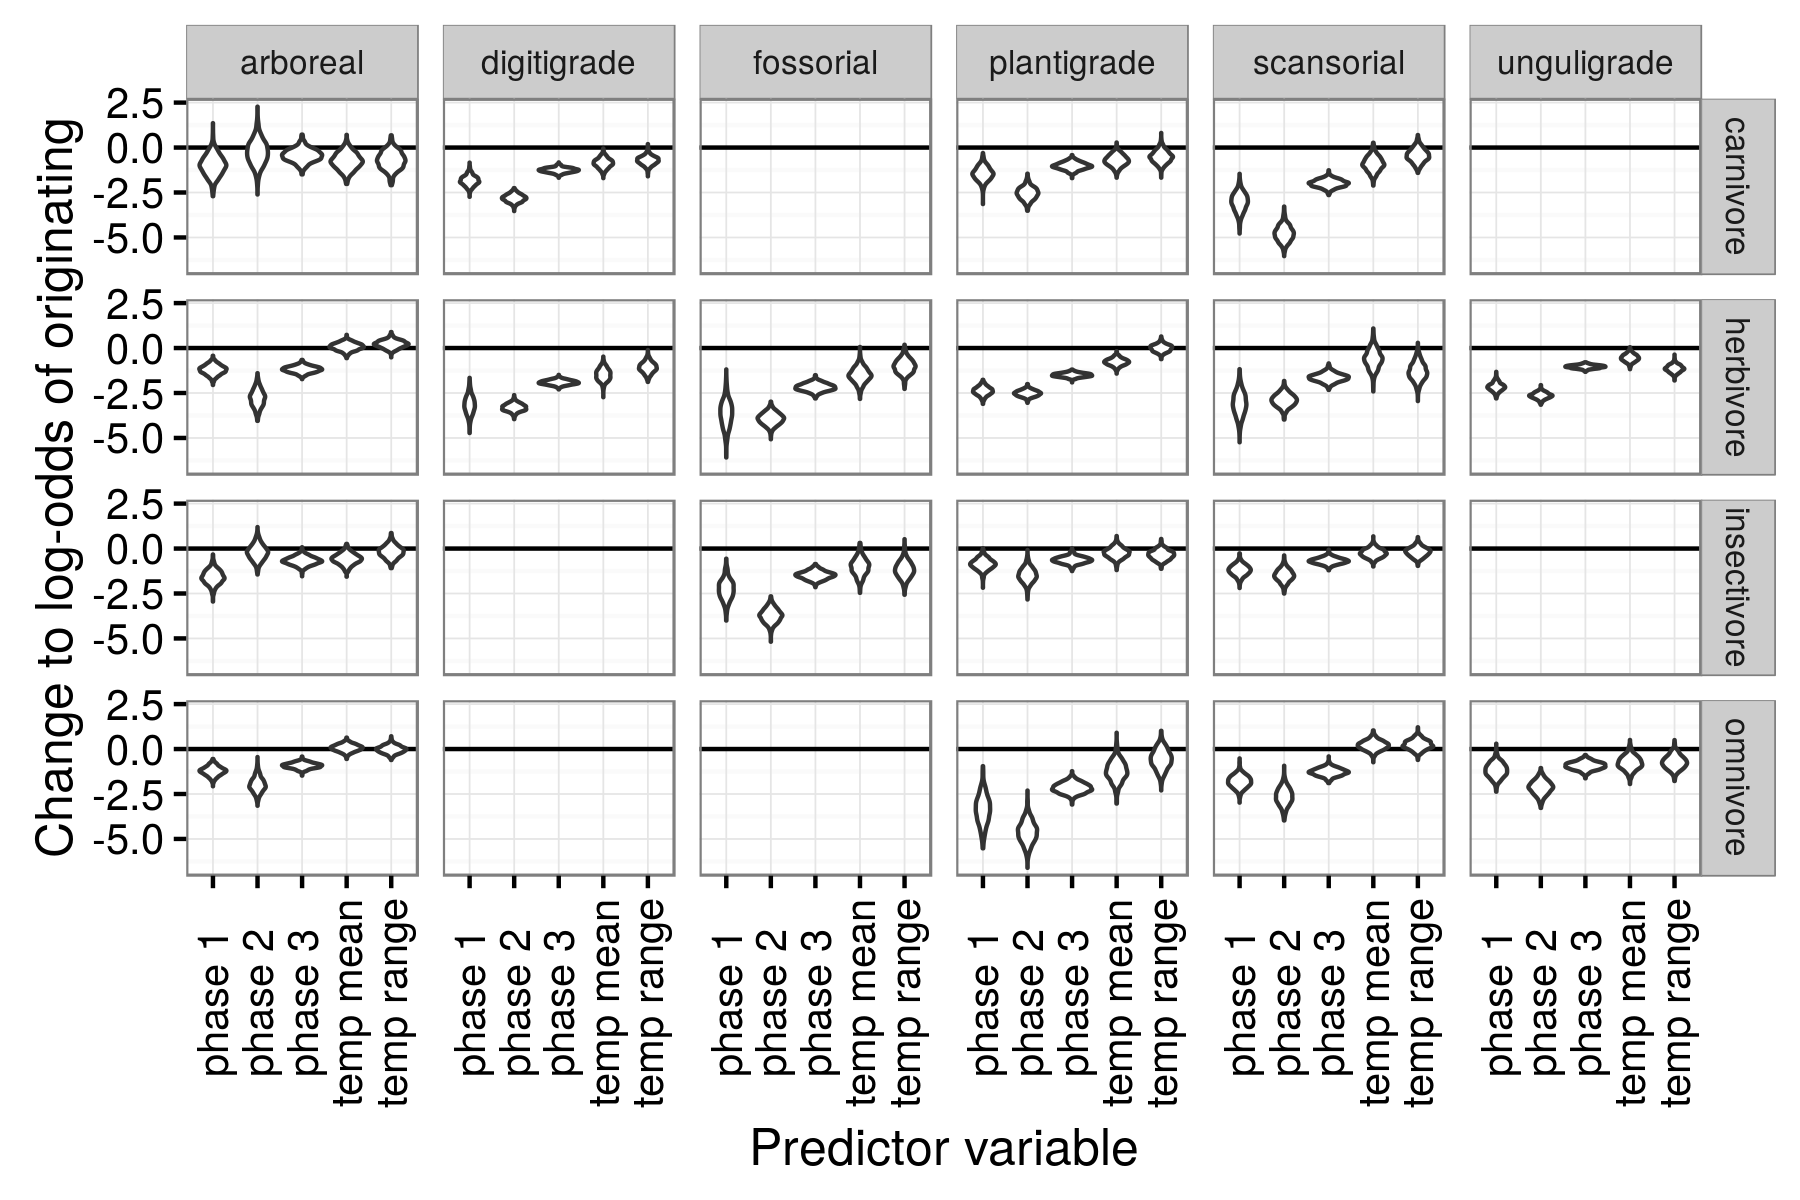
\includegraphics[width=\textwidth,height=0.4\textheight,keepaspectratio=true]{figure/group_on_origin_bd}
  \caption[Effects of group-level covariates on log-odds of ecotype origination as estimated from the the birth-death model]{Estimated effects of the group-level covariates describing environmental context on log-odds of species origination. These estimates are from the birth-death model.}
  \label{fig:group_origin_bd}
\end{figure}

\begin{figure}[ht]
  \centering
  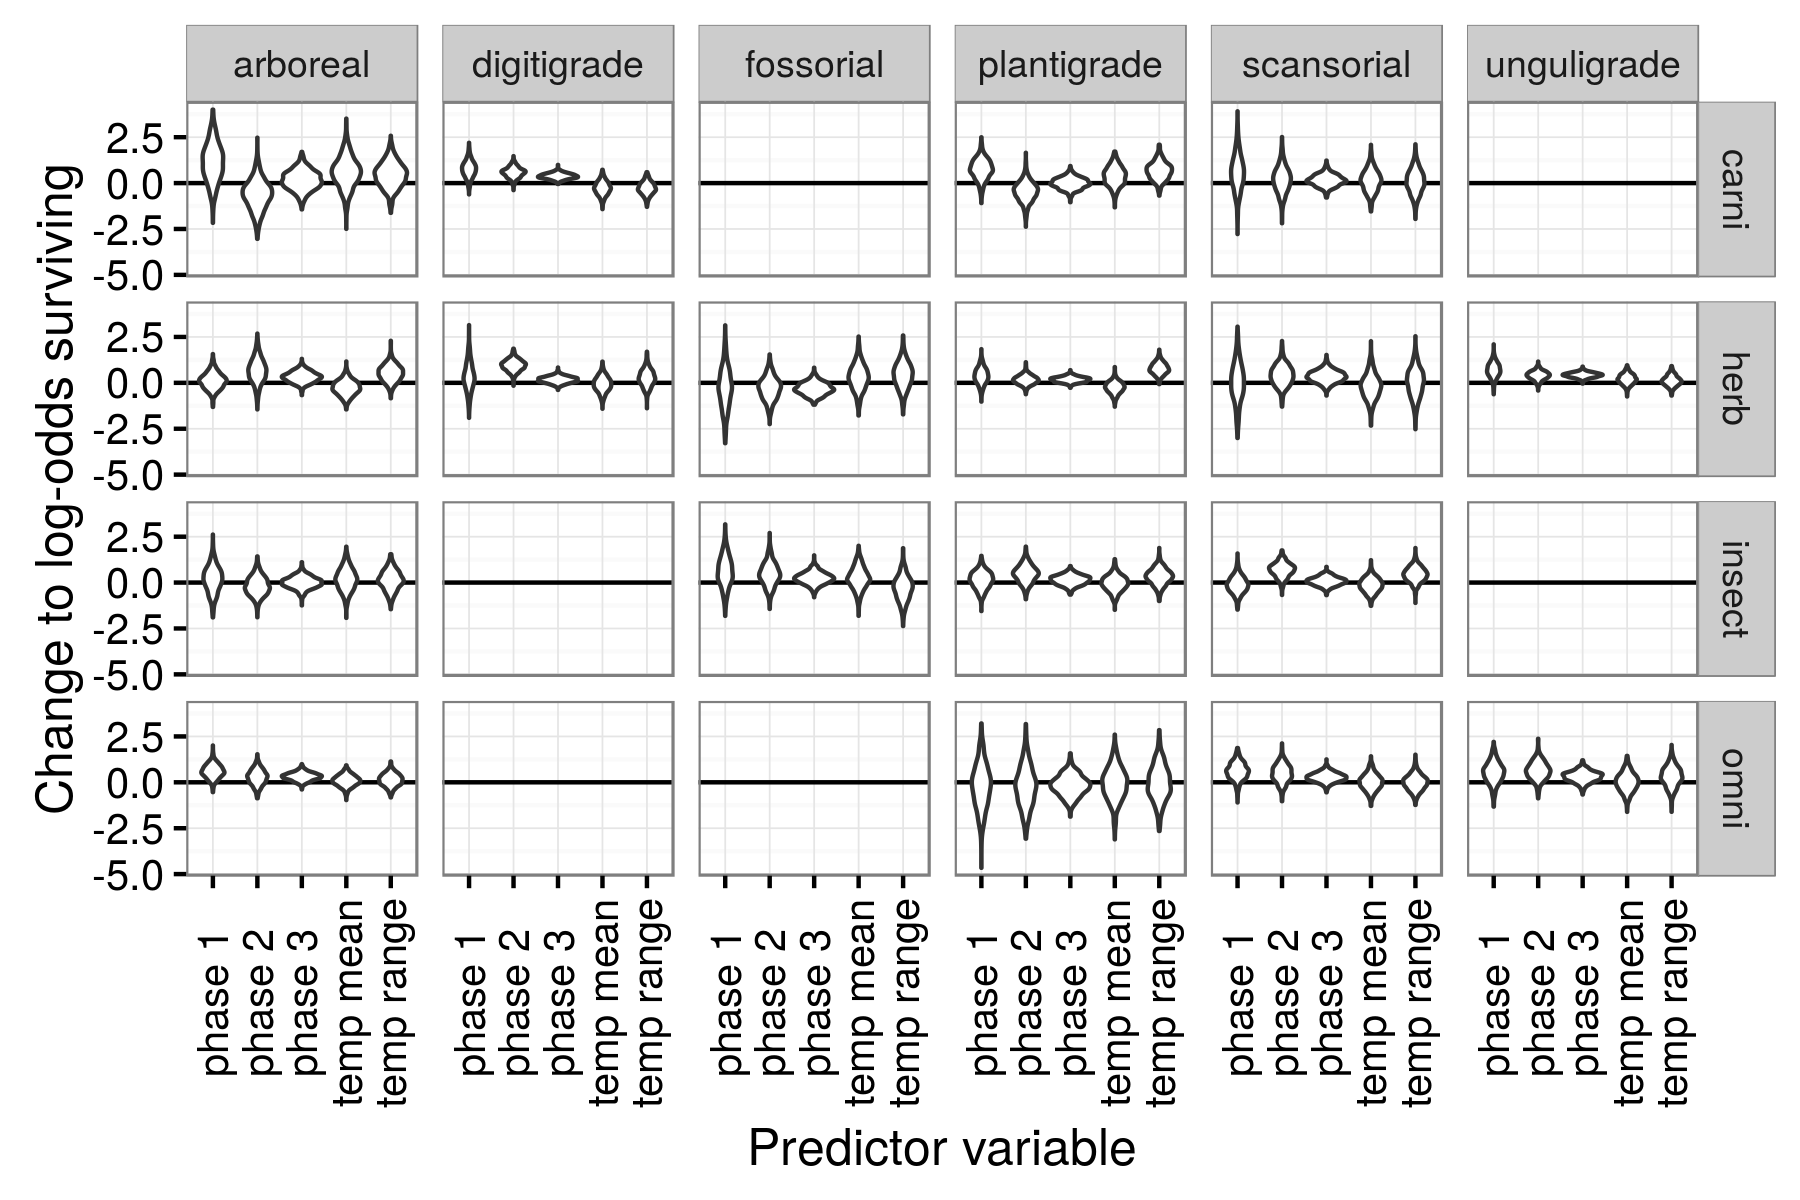
\includegraphics[width=\textwidth,height=0.4\textheight,keepaspectratio=true]{figure/group_on_survival_bd}
  \caption[Effects of group-level covariates on log-odds of ecotype survival as estimated from the the birth-death model]{Estimated effects of the group-level covariates describing environmental context on log-odds of species survlval. These estimates are from the birth-death model.}
  \label{fig:group_surv_bd}
\end{figure}




An association between plant phase and differences in the log-odds of occurrence (Fig. \ref{fig:group_pure_presence}), origination (Fig. \ref{fig:group_origin_bd}), or extinction (Fig. \ref{fig:group_surv_bd}) is interpreted to mean that if the set of possible mammal-plant interactions was either favorable (positive association) or adverse (negative association) to those ecotypes. In the case of species origination, for example, favorable conditions for an ecotype may be indicative of an increasing number of possible and available mammal-plant interactions (e.g. ecological opportunity); while adverse conditions may translate to a decreasing set of interactions or loss of appropriate environmental context. Note that favorable versus adverse condition of a plant phase is definitionally relative to the other two plant phases.

Plant phases are associated with large differences in log-odds for occurrence and origination probabilities (Tab. \ref{tab:occur_plant}), \ref{tab:origin_plant}), though there is little evidence of plant phase being an important distinguishing factor in species survival as only a few ecotypes demonstrate strong affinities with some plant phases (Tab. \ref{tab:surv_plant}). As with previous comparisons between parameter estimates associated with species occurrence and species origination, parameters associated with probability of newly originating appear as a more ``tempered'' version of those associated with probability occurrence. 

The almost universal pattern of the effect of plant phase on ecotype occurrence or origination is that the during first and last plant phases ecotypes have a greater log-odds of occurrence/origination than the second plant phase (Fig. \ref{fig:eco_occur}, \ref{fig:eco_origin}). The three exceptions to this pattern are fossorial herbivores, scansorial herbivores, and arboreal insectivores.

The difference between the third plant phase and the other two plant phases, for all ecotypes except arboreal carnivores, is obvious upon inspection the occurrence and origination time series as there is large up-tick in probability of occurring or originating towards the modern (Fig. \ref{fig:eco_occur}, \ref{fig:eco_origin}). The differences in mean probability of occurring or originating attributable to the plant phases are observable as shifts along the time series correponding to the phase barriers (Table \ref{tab:plant_def}). For example, scansorial herbivore occurrence and origination probabilities demonstrate clear shifts at 50 Mya and 16 Mya (Fig. \ref{fig:eco_occur}, \ref{fig:eco_origin}).

\begin{table}[ht]
  \centering
  \caption[Posterior probablity estimates of differences in occurrence by plant phase]{Posterior probability of the differences in the log-odds of an ecotype originating based on plant phase. These probabilities are calculated as P(Phase 1 \(>\) 2) = \( (\gamma_{phase 1} - \gamma_{phase 1} + \gamma_{phase 2}) / 100\) and similarly for the other comparisons. These estimates are from the pure-presence model.}
  \label{tab:occur_plant}
  \begin{tabular}{ l r r r }
    \hline
    & P(Phase 1 $>$ Phase 2) & P(Phase 2 $>$ Phase 3) & P(Phase 1 $>$ Phase 3) \\ 
    \hline
    arboreal carnivore & 0.460 & 0.776 & 0.866 \\ 
    digitigrade carnivore & 1.000 & 0.000 & 1.000 \\ 
    plantigrade carnivore & 1.000 & 0.040 & 1.000 \\ 
    scansorial carnivore & 1.000 & 0.001 & 1.000 \\ 
    arboreal herbivore & 1.000 & 0.540 & 1.000 \\ 
    digitigrade herbivore & 1.000 & 0.995 & 1.000 \\ 
    fossorial herbivore & 1.000 & 0.920 & 1.000 \\ 
    plantigrade herbivore & 1.000 & 0.998 & 1.000 \\ 
    scansorial herbivore & 0.999 & 0.754 & 1.000 \\ 
    unguligrade herbivore & 1.000 & 0.000 & 1.000 \\ 
    arboreal insectivore & 0.028 & 1.000 & 0.999 \\ 
    fossorial insectivore & 1.000 & 0.161 & 1.000 \\ 
    plantigrade insectivore & 0.706 & 0.774 & 0.985 \\ 
    scansorial insectivore & 0.630 & 0.937 & 1.000 \\ 
    arboreal omnivore & 0.981 & 0.165 & 0.944 \\ 
    plantigrade omnivore & 1.000 & 0.325 & 1.000 \\ 
    scansorial omnivore & 0.987 & 0.746 & 1.000 \\ 
    unguligrade omnivore & 0.990 & 0.344 & 0.997 \\ 
    \hline
  \end{tabular}
\end{table}

\begin{table}[ht]
  \centering
  \caption[Posterior probablity estimates of differences in origination by plant phase]{Posterior probability of the differences in the log-odds of an ecotype originating based on plant phase. These probabilities are calculated as P(Phase 1 \(>\) 2) = \( (\gamma_{phase 1} - \gamma_{phase 1} + \gamma_{phase 2}) / 100\) and similarly for the other comparisons. These estimates are from the birth-death model.}
  \label{tab:origin_plant}
  \begin{tabular}{ l r r r }
    \hline
    & P(Phase 1 $>$ Phase 2) & P(Phase 2 $>$ Phase 3) & P(Phase 1 $>$ Phase 3) \\ 
    \hline
    arboreal carnivore & 0.460 & 0.776 & 0.866 \\ 
    digitigrade carnivore & 1.000 & 0.000 & 1.000 \\ 
    plantigrade carnivore & 1.000 & 0.040 & 1.000 \\ 
    scansorial carnivore & 1.000 & 0.001 & 1.000 \\ 
    arboreal herbivore & 1.000 & 0.540 & 1.000 \\ 
    digitigrade herbivore & 1.000 & 0.995 & 1.000 \\ 
    fossorial herbivore & 1.000 & 0.920 & 1.000 \\ 
    plantigrade herbivore & 1.000 & 0.998 & 1.000 \\ 
    scansorial herbivore & 0.999 & 0.754 & 1.000 \\ 
    unguligrade herbivore & 1.000 & 0.000 & 1.000 \\ 
    arboreal insectivore & 0.028 & 1.000 & 0.999 \\ 
    fossorial insectivore & 1.000 & 0.161 & 1.000 \\ 
    plantigrade insectivore & 0.706 & 0.774 & 0.985 \\ 
    scansorial insectivore & 0.630 & 0.937 & 1.000 \\ 
    arboreal omnivore & 0.981 & 0.165 & 0.944 \\ 
    plantigrade omnivore & 1.000 & 0.325 & 1.000 \\ 
    scansorial omnivore & 0.987 & 0.746 & 1.000 \\ 
    unguligrade omnivore & 0.990 & 0.344 & 0.997 \\ 
    \hline
  \end{tabular}
\end{table}


\begin{table}[ht]
  \centering
  \caption[Posterior probablity estimates of differences in survival by plant phase]{Posterior probability of the differences in the log-odds of an ecotype surviving based on plant phase. These probabilities are calculated as P(Phase 1 \(>\) 2) = \( (\gamma_{phase 1} - \gamma_{phase 1} + \gamma_{phase 2}) / 100\) and similarly for the other comparisons. These estimates are from the birth-death model.}
  \label{tab:surv_plant}
  \begin{tabular}{ l r r r }
    \hline
    & P(Phase 1 $>$ Phase 2) & P(Phase 2 $>$ Phase 3) & P(Phase 1 $>$ Phase 3) \\ 
    \hline
    arboreal carnivore & 0.904 & 0.121 & 0.382 \\ 
    digitigrade carnivore & 0.181 & 0.248 & 0.004 \\ 
    plantigrade carnivore & 0.857 & 0.195 & 0.519 \\ 
    scansorial carnivore & 0.477 & 0.438 & 0.310 \\ 
    arboreal herbivore & 0.278 & 0.510 & 0.140 \\ 
    digitigrade herbivore & 0.001 & 0.978 & 0.175 \\ 
    fossorial herbivore & 0.480 & 0.723 & 0.816 \\ 
    plantigrade herbivore & 0.558 & 0.192 & 0.111 \\ 
    scansorial herbivore & 0.444 & 0.286 & 0.133 \\ 
    unguligrade herbivore & 0.548 & 0.022 & 0.002 \\ 
    arboreal insectivore & 0.691 & 0.359 & 0.492 \\ 
    fossorial insectivore & 0.334 & 0.488 & 0.221 \\ 
    plantigrade insectivore & 0.189 & 0.677 & 0.308 \\ 
    scansorial insectivore & 0.017 & 0.918 & 0.375 \\ 
    arboreal omnivore & 0.549 & 0.196 & 0.074 \\ 
    plantigrade omnivore & 0.528 & 0.537 & 0.618 \\ 
    scansorial omnivore & 0.326 & 0.442 & 0.125 \\ 
    unguligrade omnivore & 0.191 & 0.487 & 0.145 \\ 
    \hline
  \end{tabular}
\end{table}



Both aspects of global temperature analyzed here are estimated to have strong effects on species occurrence and origination for most mammal ecotypes (Tables \ref{tab:occur_temp}, \ref{tab:origin_temp}). Similarity, temperature is only expected to have a strong effect on species extinction for very few ecotypes (Tab. \ref{tab:surv_temp}). For the occurrence and origination probabilities of many ecotypes, both temperature covariates have negative estimates which means that as temperature decreases, occurrence or origination are expected to increase. The only strongly positive estimate (e.g. temperature decrease, origination decrease) is for the effect of temperature range on arboreal herbivores. Contrastingly, the only strong ecotype associations for either of the temperature covariates are with plantigrade carnivores, plantigrade herbivores, and to a less certain extent arboreal herbivores and scansorial insectivores (Tab. \ref{tab:surv_temp}). The effects of the temperature covariates on these ecotypes are all estimated to be positive (e.g. temperature range increase, increase in survival).

\begin{table}[ht]
  \centering
  \caption[Posterior probablity of effects of temperature on occurrence]{Posterior probability the the effects of the two temperature covariates on the the log-odds of an ecotype occurring are greater than 0. What is estimated is the probability that these estimates are greater than 0; high or low probabilities indicate the ``strength'' of the covariate in that direction (positive and negative, respectively). These estimates are from the pure-presence model.}
  \label{tab:occur_temp}
  \begin{tabular}{ l r r }
    \hline
    & \(P(\gamma_{temp\ mean} > 0)\) & \(P(\gamma_{temp\ range} > 0)\) \\ 
    \hline
    arboreal carnivore & 0.169 & 0.317 \\ 
    digitigrade carnivore & 0.000 & 0.000 \\ 
    plantigrade carnivore & 0.168 & 0.304 \\ 
    scansorial carnivore & 0.000 & 0.206 \\ 
    arboreal herbivore & 0.943 & 0.969 \\ 
    digitigrade herbivore & 0.000 & 0.000 \\ 
    fossorial herbivore & 0.001 & 0.022 \\ 
    plantigrade herbivore & 0.000 & 0.832 \\ 
    scansorial herbivore & 0.009 & 0.003 \\ 
    unguligrade herbivore & 0.000 & 0.000 \\ 
    arboreal insectivore & 0.006 & 0.783 \\ 
    fossorial insectivore & 0.016 & 0.003 \\ 
    plantigrade insectivore & 0.127 & 0.260 \\ 
    scansorial insectivore & 0.009 & 0.238 \\ 
    arboreal omnivore & 0.337 & 0.191 \\ 
    plantigrade omnivore & 0.012 & 0.120 \\ 
    scansorial omnivore & 0.597 & 0.935 \\ 
    unguligrade omnivore & 0.002 & 0.002 \\ 
    \hline
  \end{tabular}
\end{table}



\begin{table}[ht]
  \centering
  \caption[Posterior probablity of effects of temperature on origination]{Posterior probability that the effects of the two temperature covariates on the the log-odds of an ecotype origination are greater than 0. What is estimated is the probability that these estimates are greater than 0; high or low probabilities indicate the ``strength'' of the covariate in that direction (positive and negative, respectively). These estimates are from the birth-death model.}
  \label{tab:origin_temp}
  \begin{tabular}{ l r r }
    \hline
    & \(P(\gamma_{temp\ mean} > 0)\) & \(P(\gamma_{temp\ range} > 0)\) \\ 
    \hline
    arboreal carnivore & 0.086 & 0.045 \\ 
    digitigrade carnivore & 0.001 & 0.000 \\ 
    plantigrade carnivore & 0.013 & 0.054 \\ 
    scansorial carnivore & 0.007 & 0.062 \\ 
    arboreal herbivore & 0.853 & 0.957 \\ 
    digitigrade herbivore & 0.000 & 0.001 \\ 
    fossorial herbivore & 0.000 & 0.002 \\ 
    plantigrade herbivore & 0.000 & 0.428 \\ 
    scansorial herbivore & 0.106 & 0.003 \\ 
    unguligrade herbivore & 0.000 & 0.000 \\ 
    arboreal insectivore & 0.028 & 0.314 \\ 
    fossorial insectivore & 0.010 & 0.006 \\ 
    plantigrade insectivore & 0.188 & 0.090 \\ 
    scansorial insectivore & 0.182 & 0.224 \\ 
    arboreal omnivore & 0.749 & 0.482 \\ 
    plantigrade omnivore & 0.007 & 0.117 \\ 
    scansorial omnivore & 0.765 & 0.699 \\ 
    unguligrade omnivore & 0.016 & 0.023 \\ 
    \hline
  \end{tabular}
\end{table}

\begin{table}[ht]
  \centering
  \caption[Posterior probablity of effects of temperature on survival]{Posterior probability that the effects of the two temperature covariates on the the log-odds of an ecotype survival are greater than 0. What is estimated is the probability that these estimates are greater than 0; high or low probabilities indicate the ``strength'' of the covariate in that direction (positive and negative, respectively). These estimates are from the birth-death model.}
  \label{tab:surv_temp}
  \begin{tabular}{ l r r }
    \hline
    & \(P(\gamma_{temp\ mean} > 0)\) & \(P(\gamma_{temp\ range} > 0)\) \\ 
    \hline
    arboreal carnivore & 0.777 & 0.745 \\ 
    digitigrade carnivore & 0.236 & 0.211 \\ 
    plantigrade carnivore & 0.763 & 0.929 \\ 
    scansorial carnivore & 0.596 & 0.554 \\ 
    arboreal herbivore & 0.261 & 0.878 \\ 
    digitigrade herbivore & 0.438 & 0.720 \\ 
    fossorial herbivore & 0.676 & 0.731 \\ 
    plantigrade herbivore & 0.215 & 0.997 \\ 
    scansorial herbivore & 0.377 & 0.535 \\ 
    unguligrade herbivore & 0.768 & 0.655 \\ 
    arboreal insectivore & 0.614 & 0.610 \\ 
    fossorial insectivore & 0.673 & 0.337 \\ 
    plantigrade insectivore & 0.470 & 0.787 \\ 
    scansorial insectivore & 0.364 & 0.879 \\ 
    arboreal omnivore & 0.620 & 0.645 \\ 
    plantigrade omnivore & 0.476 & 0.484 \\ 
    scansorial omnivore & 0.514 & 0.494 \\ 
    unguligrade omnivore & 0.513 & 0.729 \\ 
    \hline
  \end{tabular}
\end{table}





\subsection*{Analysis of diversity}

All of the analyses of diversification and macroevolutionary rates has been done using only the birth-death model because of the model's better posterior predictive check performance (Fig. \ref{fig:ppc}).


The general pattern of the estimated North American total mammal diversity for the Cenozoic is ``stable'' in that mean standing diversity does not fluctuate wildly and rapidly over the Cenozoic (Fig. \ref{fig:diversity_est}). In broad strokes, the first 15 or so million years of the Cenozoic are characterized by a gradual decline in standing diversity until approximately 45-50 million years ago (early-middle Eocene). Following this decline, standing diversity is broadly constant from 45 to 18 Mya (early Miocene). After this, there is a rapid spike in diversity followed by a slight decline in diversity up to the Modern. This characterization of the estimated diversity history is knowingly broad strokes and diversity time series is not without variation and vagaries.

When viewed through the lens of diversification rate, some of the structure behind the estimated diversity history begins to take shape (Fig. \ref{fig:diversity_rate}). For most of the Cenozoic, the diversification rate hovers around zero, punctuated by both positive and negative spikes. The largest spike in diversification rate is at 18 Mya, which is early Oligocene (Fig. \ref{fig:diversity_rate}). Other notable increases in diversification rate occur 56, 46, 38, and 6 Mya (Table \ref{tab:div_peak}), though the last of these may be due edge effects surrounding the partial-identifiability of \(p_{t = T}\) . Notable decreases in diversification rate occur 60, 54, 50, 44, 34, 20, 16, 12, and 8 Mya (Table \ref{tab:div_peak}), meaning that diversification rate has more major decreases than increases. Given that diversification rate more closely resembles origination rate than extinction rate (Fig. \ref{fig:diversity_rate}, \ref{fig:origin_rate}, \ref{fig:extinct_rate}), these decreases in diversification rate may be indicative of ``depletions'' (failure to replace extinct taxa) rather than pulses of extinction.

The comparison between per capita origination and extinction rate estimates reveals how diversification rate is formed (Fig. \ref{fig:origin_rate}, \ref{fig:extinct_rate}). As expected given previous inspection of the ecotype specific estimates of origination and survival probabilities from the birth-death model, diversification rate seems most driven by changes in origination rate as opposed to extinction rate. Extinction rate, on the other hand, demonstrates an almost saw-toothed pattern around a constant mean (Fig. \ref{fig:extinct_rate})>


\begin{figure}[ht]
  \begin{subfigure}[b]{0.45\textwidth}
    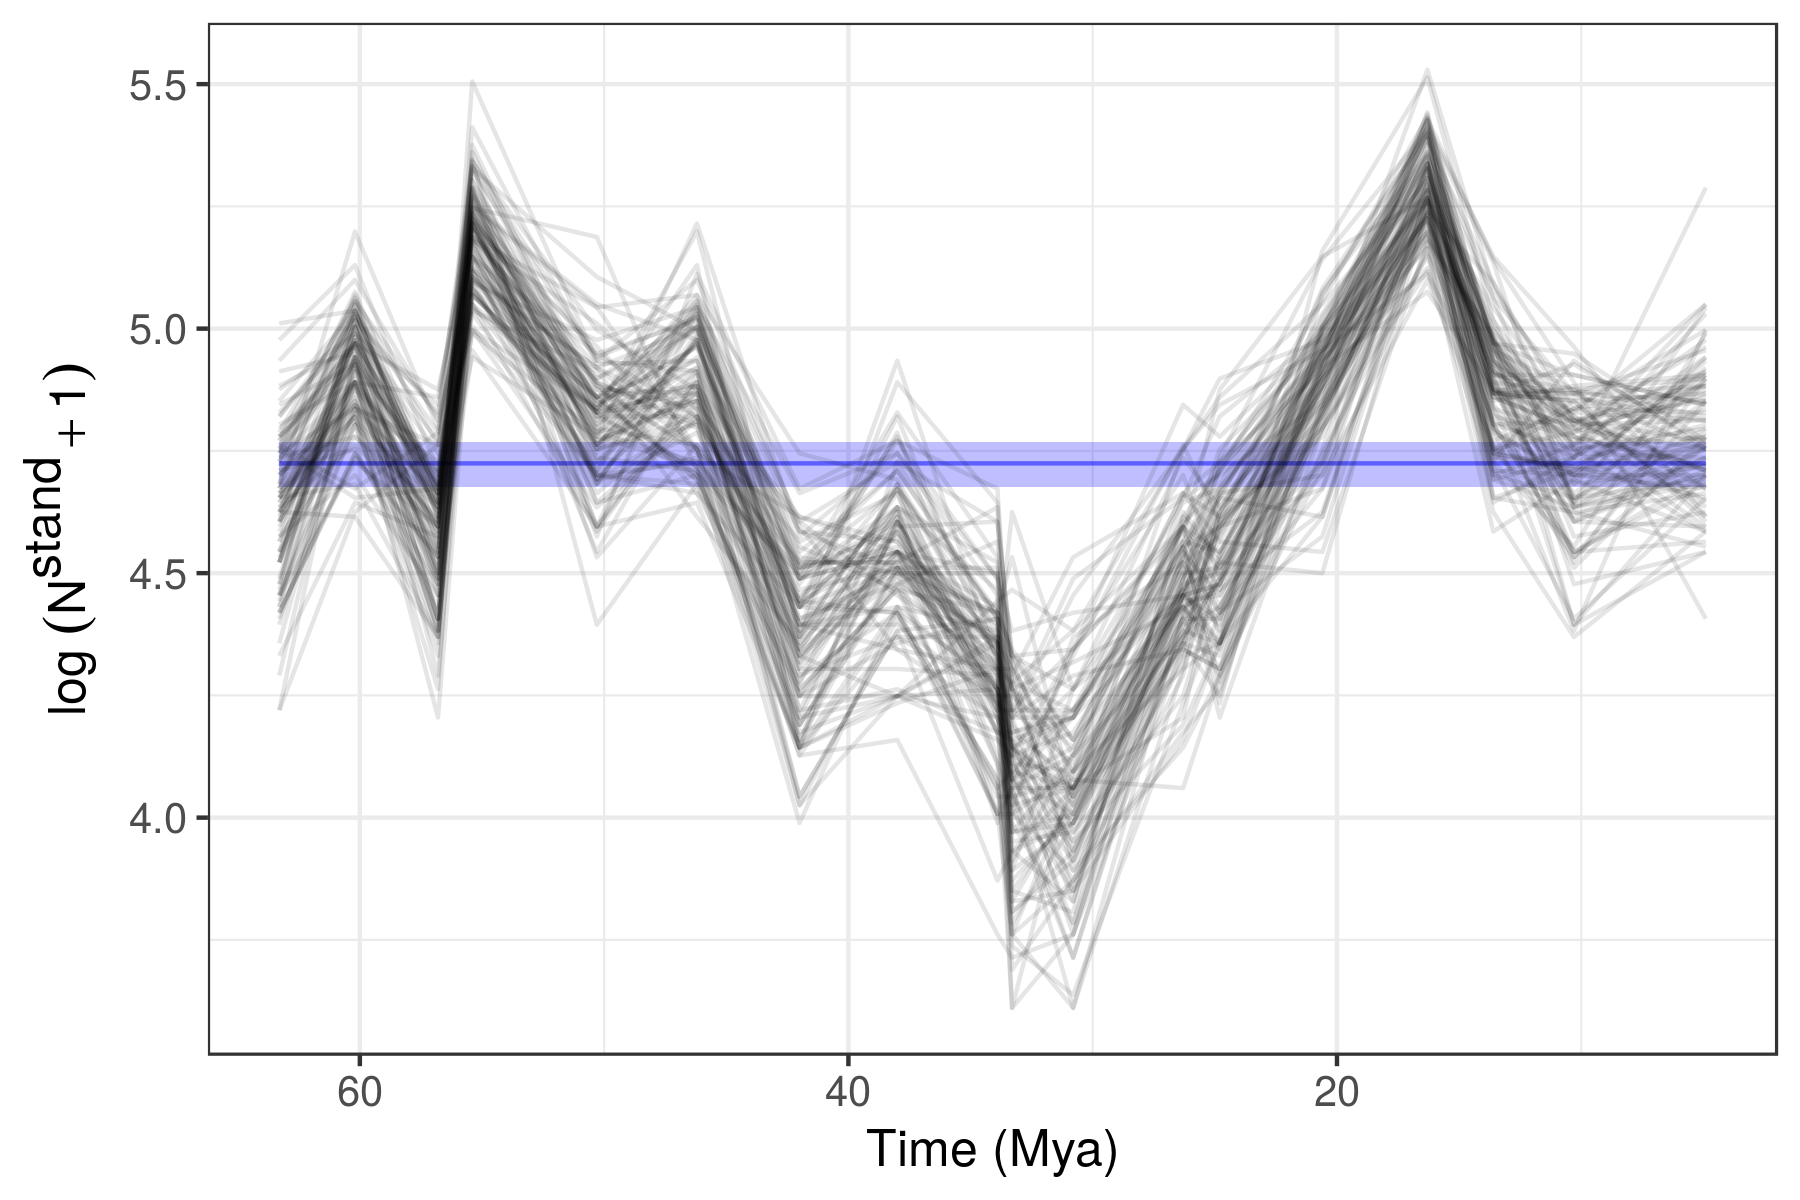
\includegraphics[width=\textwidth,height=0.4\textheight,keepaspectratio=true]{figure/log_diversity}
    \caption{Log diversity}
    \label{fig:diversity_est}
  \end{subfigure}
  \begin{subfigure}[b]{0.45\textwidth}
    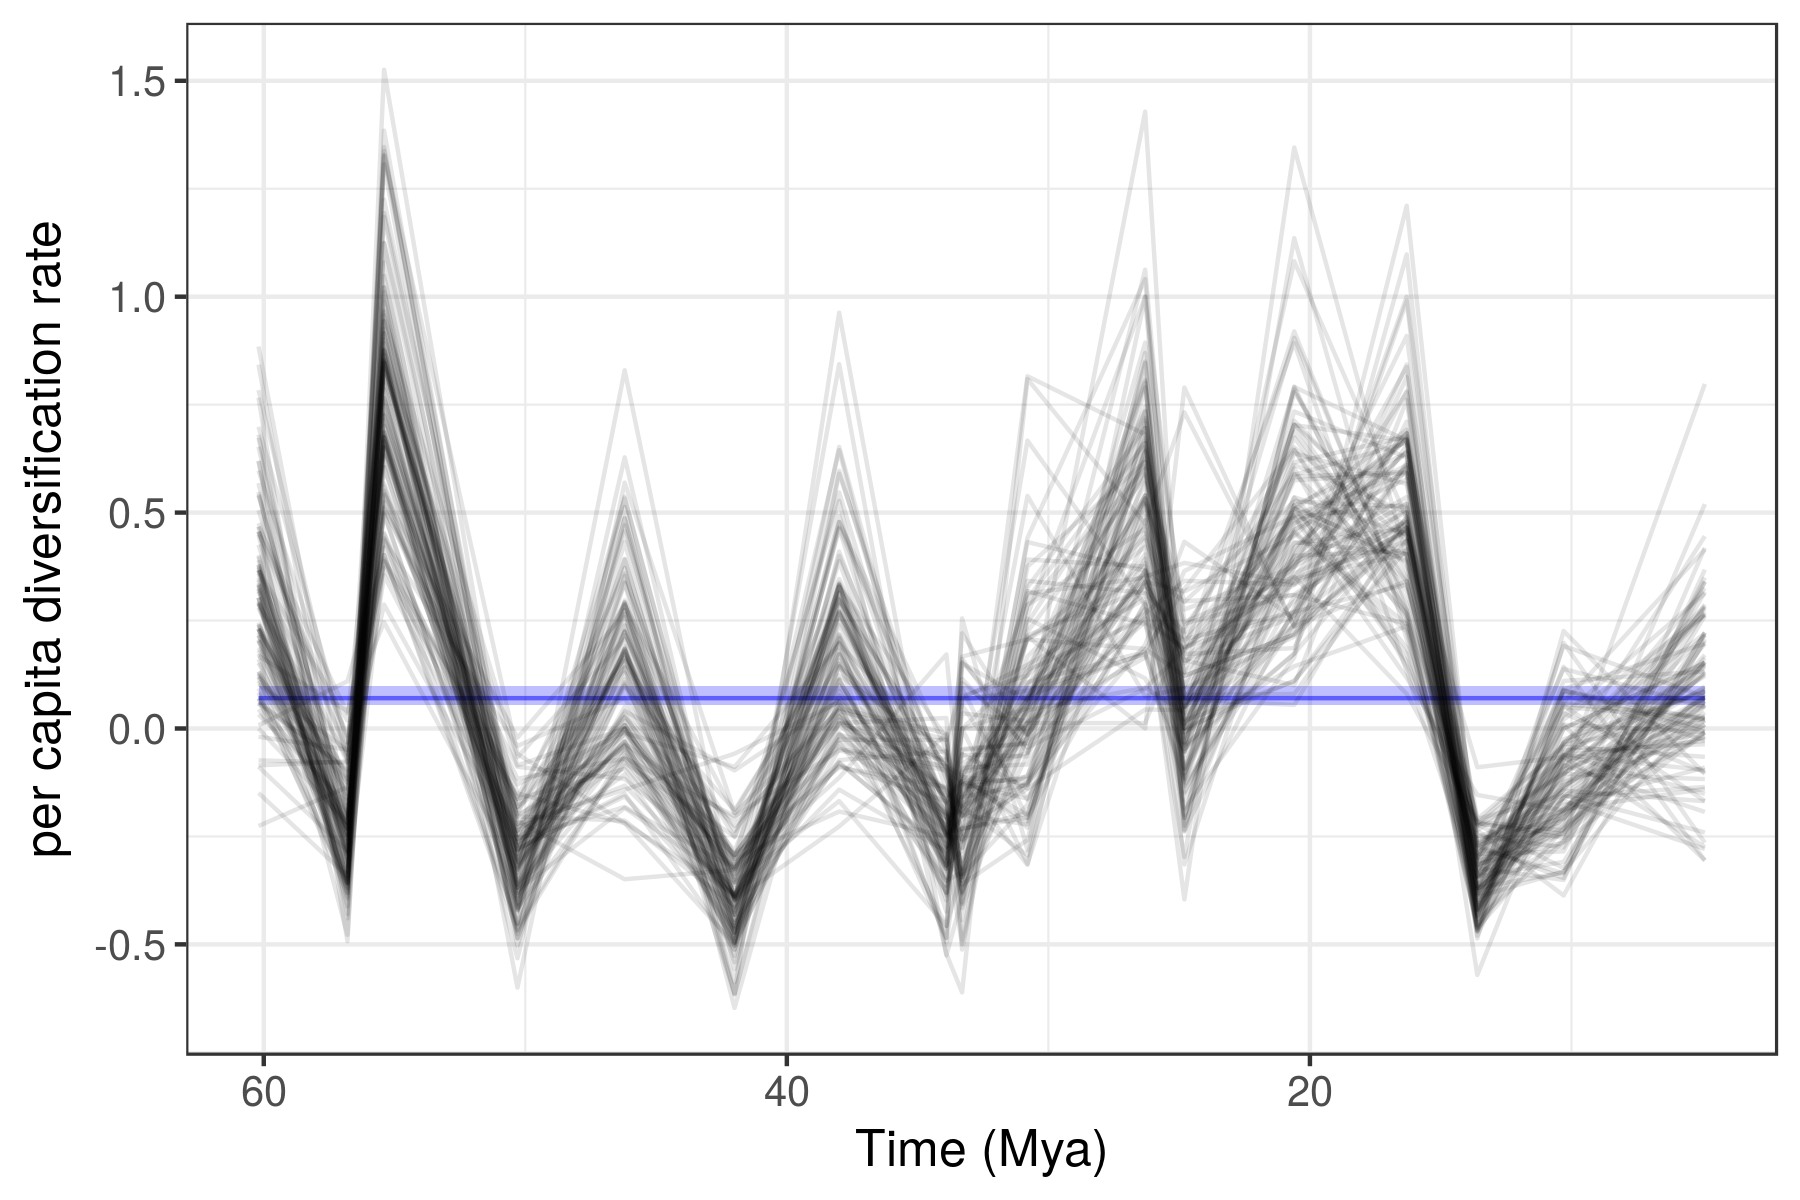
\includegraphics[width=\textwidth,height=0.4\textheight,keepaspectratio=true]{figure/div_rate}
    \caption{Diversification rate}
    \label{fig:diversity_rate}
  \end{subfigure}

  \begin{subfigure}[b]{0.45\textwidth}
    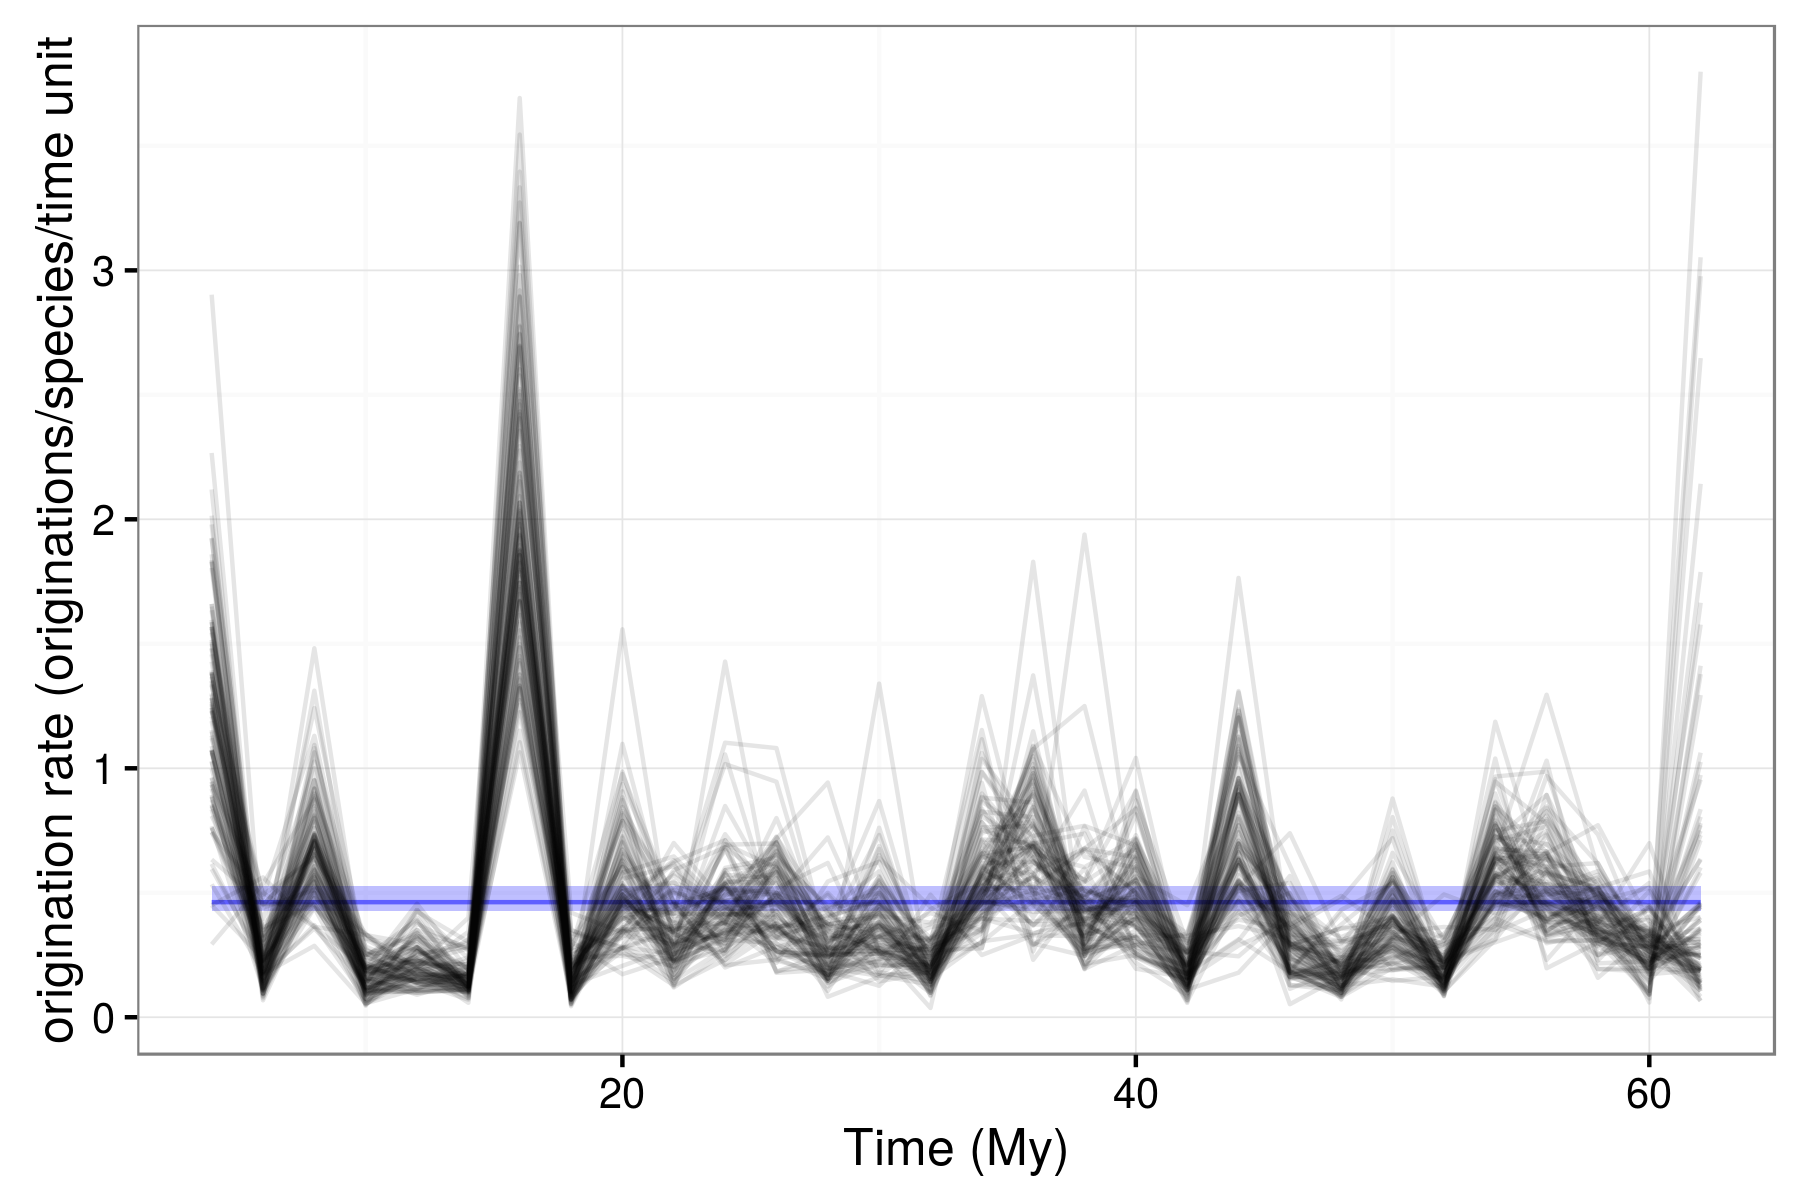
\includegraphics[width=\textwidth,height=0.4\textheight,keepaspectratio=true]{figure/orig_rate}
    \caption{Origination rate}
    \label{fig:origin_rate}
  \end{subfigure}
  \begin{subfigure}[b]{0.45\textwidth}
    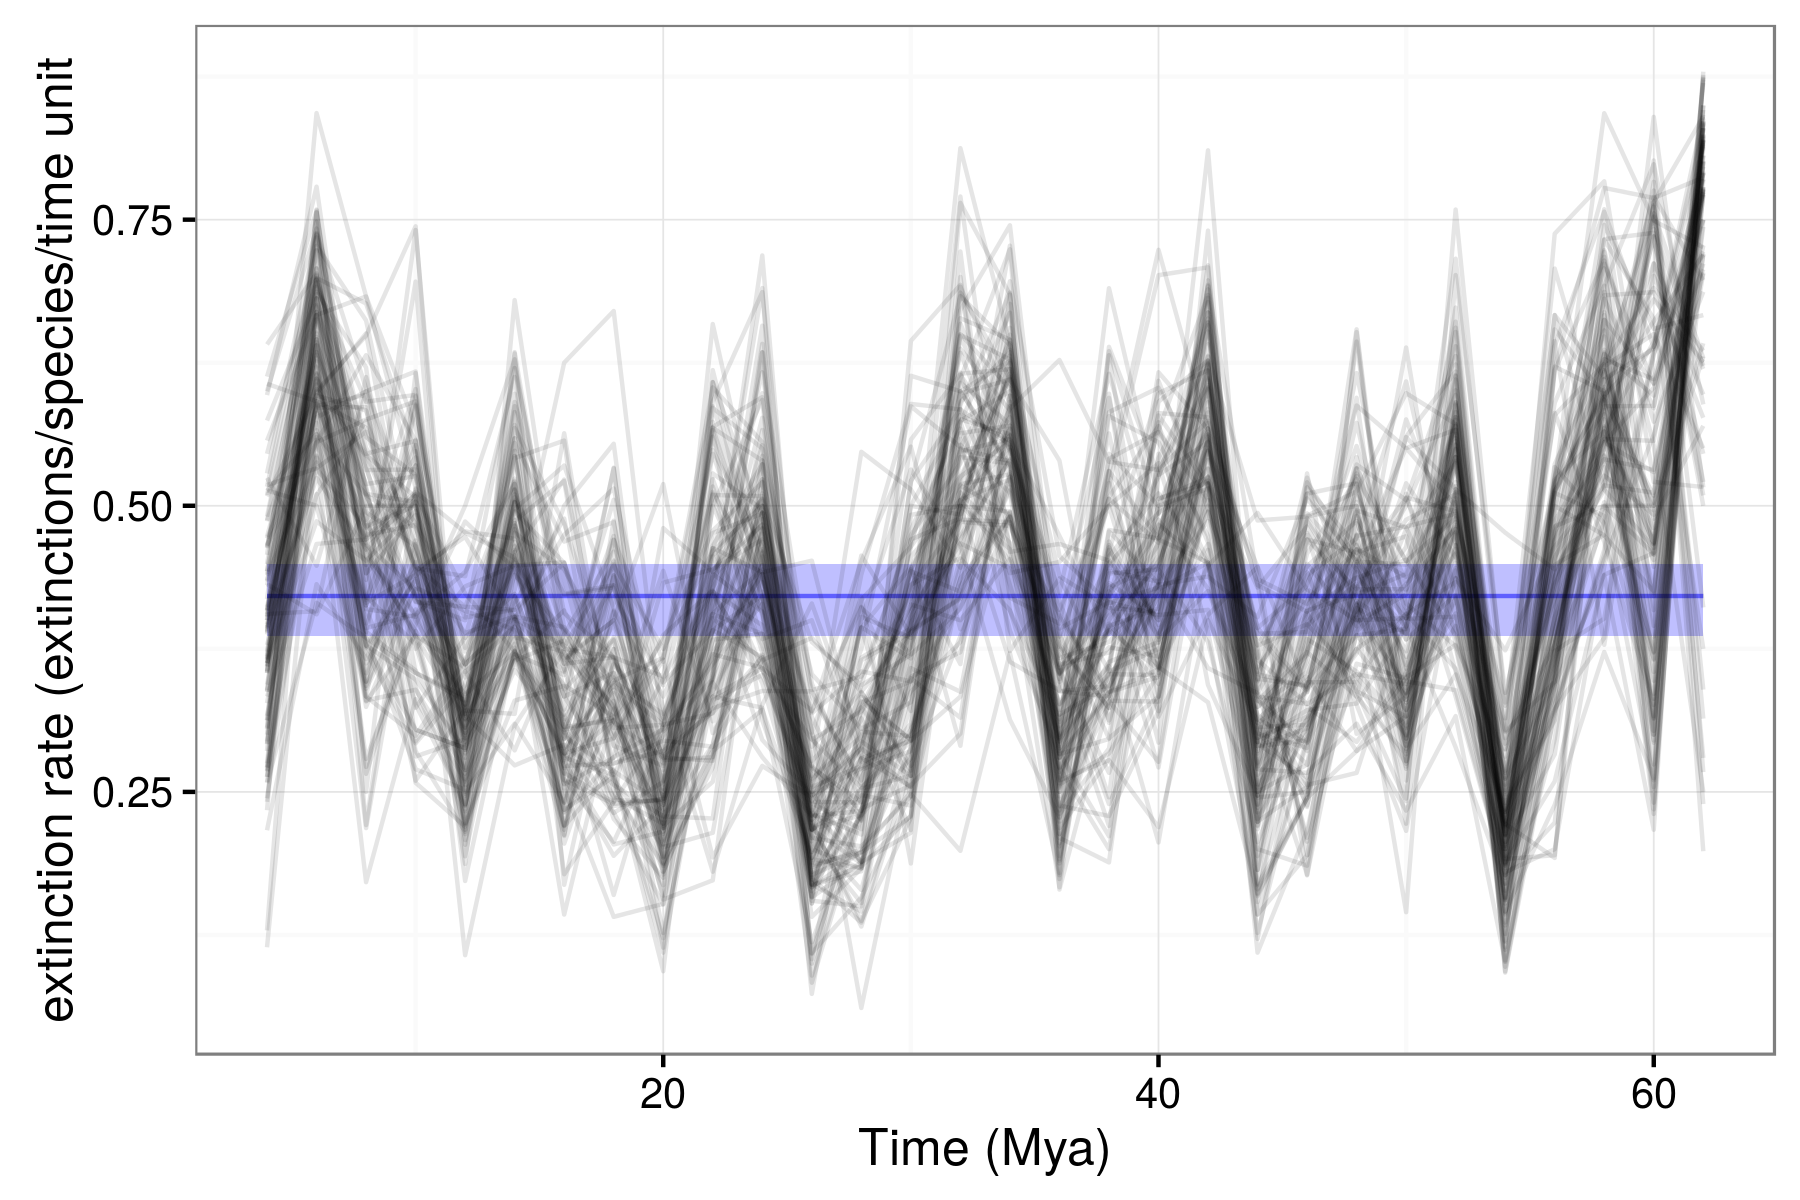
\includegraphics[width=\textwidth,height=0.4\textheight,keepaspectratio=true]{figure/death_rate}
    \caption{Extinction rate}
    \label{fig:extinct_rate}
  \end{subfigure}
  \caption[Estimated mammal log-diversity and macroevolutionary rates for the Cenozoic]{Posterior estimates of the time series of Cenozoic North American mammal diversity and it's characteristic macroevolutionary rates; all estimates are from the birth-death model and 100 posterior draws are plotted to indicate the uncertainty in these estimates. The blue horizontal strip corresponds to the 80\% credible interval of estimated mean standing diversity, diversification rate, origination rate, and extinction rate respectively; the median esimate is also indicated. What is also plotted is the  The dramatic differences between diversity estimates at the first and second time points and the penultimate and last time points in this series are caused by well known edge effects in discrete-time birth-death models caused by \(p_{\_, t = 1}\) and \(p_{\_, t = T}\) being partially unidentifiable \citep{Royle2008}; the hierarchical modeling strategy used here helps mitigate these effects but they are still present \citep{Gelman2013d,Royle2008}. Diversification rate is in units of species gained per species present per time unit (2 My), origination rate is in units of species originating per species present per time unit, and extinction rate is in units of species becoming extinct per species present per time unit.}
  \label{fig:macro_values}
\end{figure}

\begin{table}[ht]
  \centering
  \caption[Posterior probability estimates of a peak in diversity, diversification]{Posterior probabilities of diversity \(N^{stand}_{t}\) or diversification rate \(D^{rate}_{t}\) being greater than average standing diversity \(\overline{N^{stand}}\) or average diversification rate \(\overline{D^{rate}}\) for the whole Cenozoic. The ``Time'' column corresponds to the top of each of the temporal bins. Diversification rate can not be estimated for the last time point because it is unknown how many more species originated or went extinct following this tempral bin. The estimates are from the birth-death model.}
  \label{tab:div_peak}
  \begin{tabular}{ r r r }
    \hline
    Time (Mya) & \(P(N^{stand}_{t} > \overline{N^{stand}})\) & \(P(D^{rate}_{t} > \overline{D^{rate}})\) \\ 
    \hline
    64.00 & 0.99 & 0.18 \\ 
    62.00 & 0.93 & 0.15 \\ 
    60.00 & 0.93 & 0.04 \\ 
    58.00 & 0.53 & 0.59 \\ 
    56.00 & 0.72 & 0.99 \\ 
    54.00 & 0.99 & 0.00 \\ 
    52.00 & 0.59 & 0.45 \\ 
    50.00 & 0.57 & 0.01 \\ 
    48.00 & 0.05 & 0.27 \\ 
    46.00 & 0.04 & 0.92 \\ 
    44.00 & 0.53 & 0.00 \\ 
    42.00 & 0.01 & 0.44 \\ 
    40.00 & 0.00 & 0.37 \\ 
    38.00 & 0.01 & 0.94 \\ 
    36.00 & 0.23 & 0.46 \\ 
    34.00 & 0.22 & 0.01 \\ 
    32.00 & 0.00 & 0.31 \\ 
    30.00 & 0.00 & 0.33 \\ 
    28.00 & 0.00 & 0.83 \\ 
    26.00 & 0.03 & 0.32 \\ 
    24.00 & 0.02 & 0.25 \\ 
    22.00 & 0.01 & 0.89 \\ 
    20.00 & 0.15 & 0.02 \\ 
    18.00 & 0.02 & 1.00 \\ 
    16.00 & 1.00 & 0.00 \\ 
    14.00 & 0.83 & 0.11 \\ 
    12.00 & 0.67 & 0.01 \\ 
    10.00 & 0.11 & 0.79 \\ 
    8.00 & 0.40 & 0.02 \\ 
    6.00 & 0.00 & 0.98 \\ 
    4.00 & 0.59 & \\ 
    \hline
  \end{tabular}
\end{table}


Diversity partitioned by ecotype reveals a lot of the complexity behind the pattern of mammal diversity for the Cenozoic (Fig. \ref{fig:ecotype_diversity}). 

\begin{figure}[ht]
  \centering
  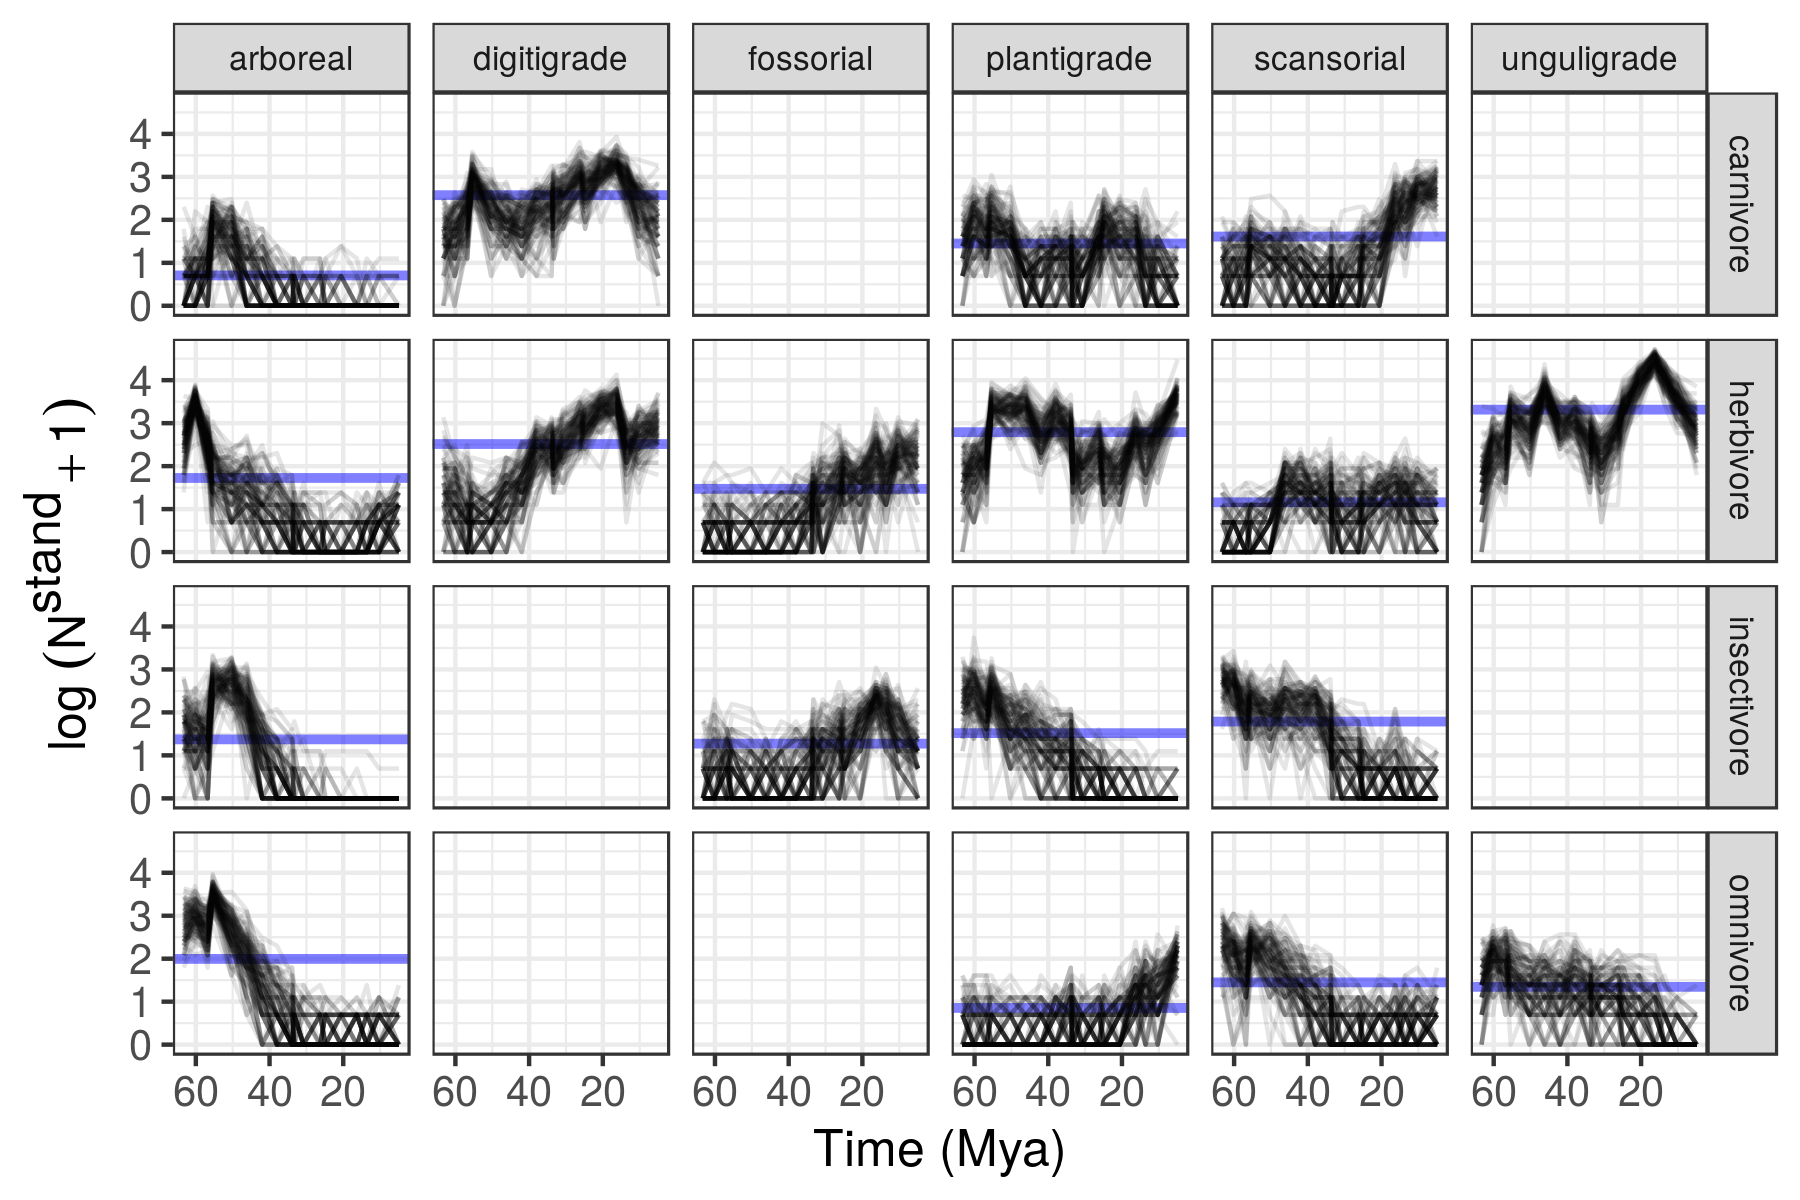
\includegraphics[width=\textwidth,height=0.4\textheight,keepaspectratio=true]{figure/ecotype_diversity}
  \caption[Estimated mammal ecotype log-diversity for the Cenozoic]{Posterior of standing log-diversity of North American mammals by ecotype for the Cenozoic as estimated from the birth-death model; 100 posterior draws are plotted to indicate the uncertainty in these estimates and what is technically plotted is log of diversity plus 1.}
  \label{fig:ecotype_diversity}
\end{figure}

Arboreal ecotypes obtain peak diversity early in the Cenozoic and then decline for the rest of the time series, becoming increasingly rare or absent as diversity approaches the Modern (Fig. \ref{fig:ecotype_diversity}). Arboreal herbivores and omnivores obtain peak diversity at the beginning of the Cenozoic then go into decline while remaining a small part of the species pool, while arboreal carnivores and insectivores obtain peak diversity 52-50 Mya and then quickly decline and become extremely rare or entirely absent from the species pool.

The diversity of both digitigrade and unguligrade herbivores increase over the Cenozoic (Fig. \ref{fig:ecotype_diversity}). In contrast, plantigrade herbivore diversity does not have a single, broad-strokes pattern; instead, diversity increases, decreases, and may have then increased till the Modern. Contrastingly, fossorial and scansorial herbivores demonstrate a much flatter history of diversity, with a slight increase in diversity that over time is more pronounced among fossorial taxa than scansorial taxa.

Digitigrade carnivores have a multi-modal diversity history, with peaks 54-52 and 12-10 Mya (Fig.\ref{fig:ecotype_diversity}). Between these two peaks digitigrade carnivore diversity dips below average diversity following the first peak and then grows slowly until the second peak. Plantigrade carnivores obtain peak diversity in the early Cenozoic and then maintain a relatively stable diversity until another peak at the end of the Cenozoic. 

There are some broad similarities in diversity histories of insectivorous and omnivorous taxa. The diversity histories of arbreal, plantigrade, and scansorial insectivorous taxa all demonstrate a decreasing pattern with time, while fossorial insectivores have a flat diversity history with a peak approximately 10 Mya (Fig. \ref{fig:ecotype_diversity}). Arboreal and scansorial omnivores decrease in diversity from their initial peaks early in the Cenozoic, and plantigrade omnivores have a generally flat diversity history with a sudden peak in diversity late in the Cenozoic (Fig. \ref{fig:ecotype_diversity}). Unguligrade omnivores also demonstrate a possible decrease in diversity over the Cenozoic, but not as clearly as arboreal and scansorial omnivores.

Many of the estimated ecotype specific diversity histories share a similar increases in diversity to one degree or another at the late Cenozoic 16-14 Mya (Fig. \ref{fig:ecotype_diversity}); these increases are either sustained or temporary: digitigrade carnivores, plantigrade carnivores, scansorial carnivores, unguligrade herbivores, fossorial insectivores, and plantigrade omnivores.

When ecotype diversity is decomposed into the number of origination events per time bin (Fig. \ref{fig:ecotype_birth}) and the number of extinction events per time bin (Fig. \ref{fig:ecotype_death}) the estimates are clearly similar; there are no obvious major cross-ecotype origination or extinction events, and there is no evidence of a sudden turnover as expected peaks in originations proceed peaks in peaks in the number of extinctions. Also, it is clear that the sustained increases in digitigrade and unguligrade herbivore diversity observed above (Fig. \ref{fig:ecotype_diversity}) is driven by an increase in the average number of originations as with a relatively constant number of extinctions over time (Fig. \ref{fig:ecotype_birth}, \ref{fig:ecotype_death}).


\begin{figure}[ht]
  \centering
  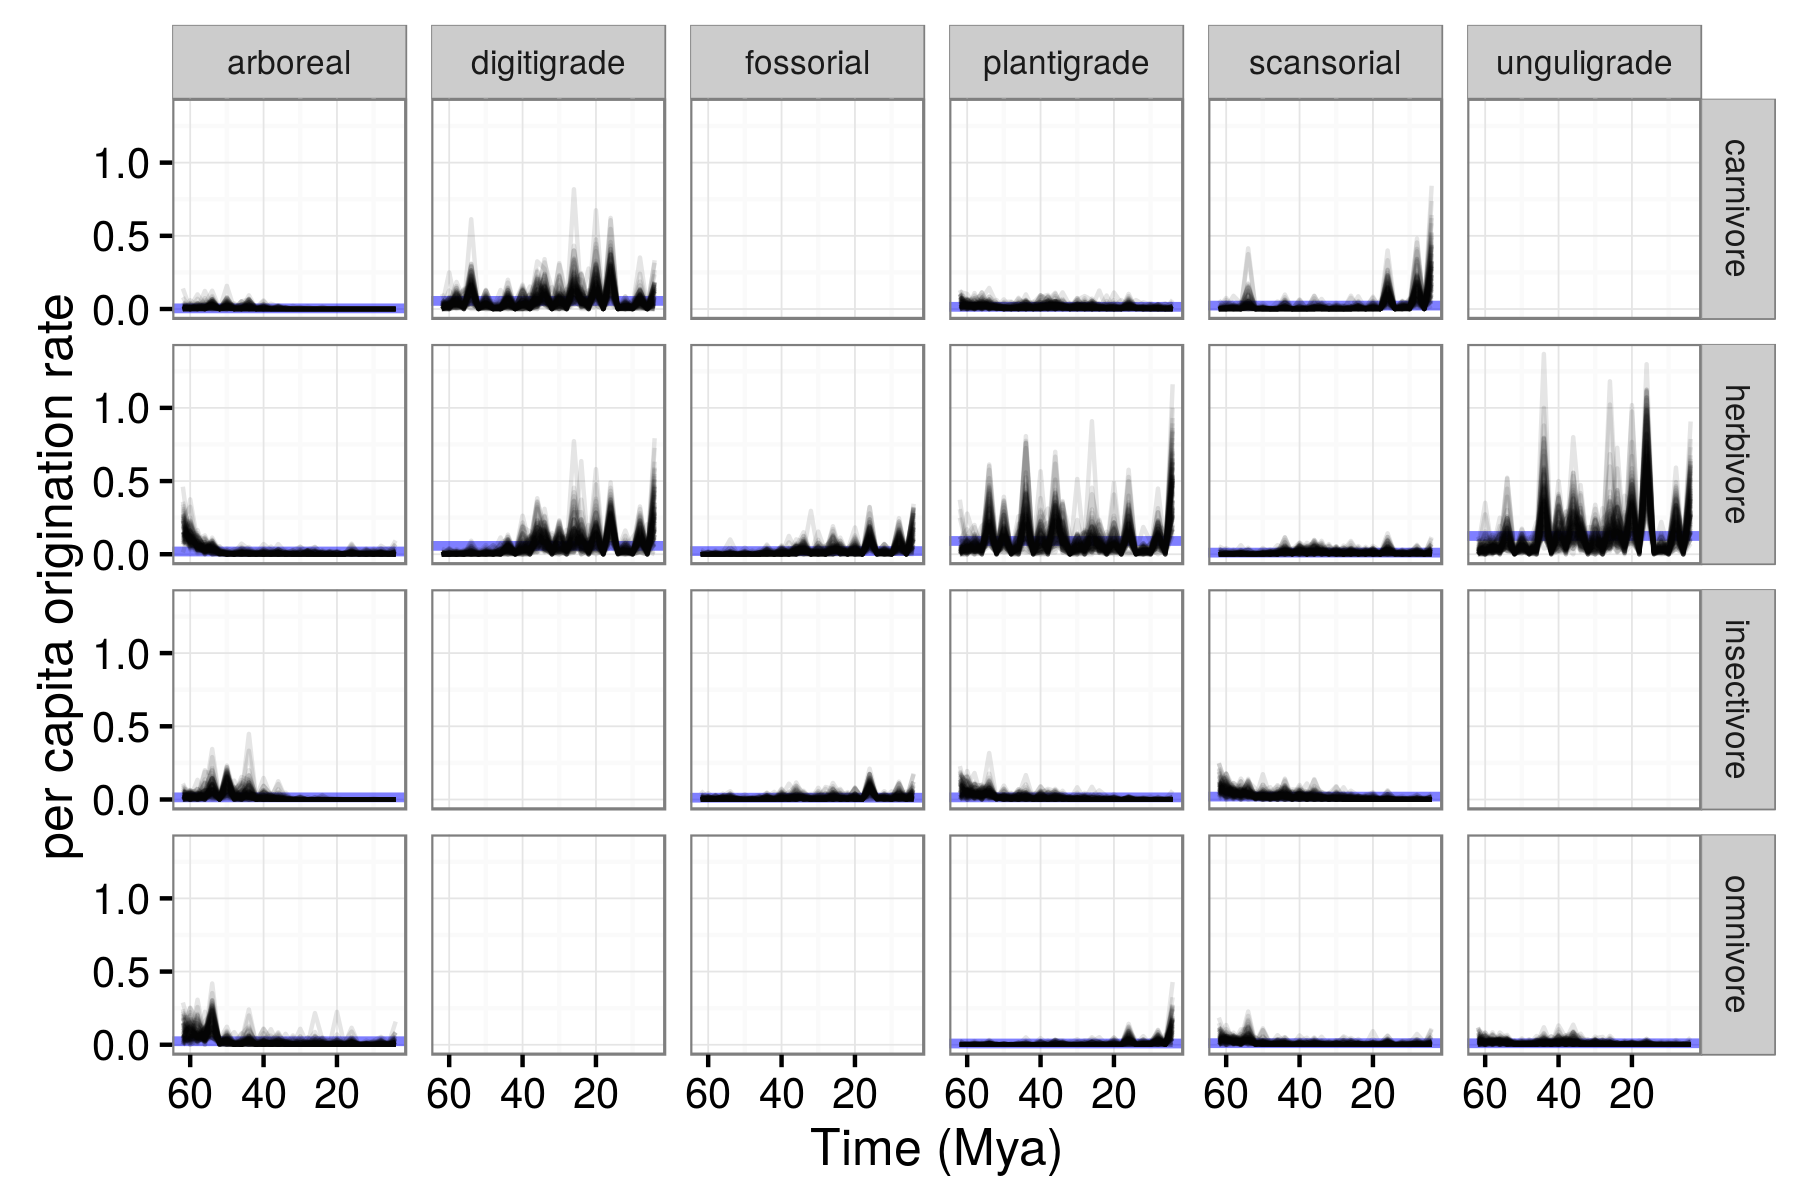
\includegraphics[width=\textwidth,height=0.4\textheight,keepaspectratio=true]{figure/birth_eco}
  \caption[Estimated number of origination events by mammal ecotype]{Posterior estimates of the number of origination events from one temporal bin to another, plotted at the bin they originate from. 100 posterior draws are plotted to indicate the uncertainty in these estimates. Also, what is ploted is log of the number of originations plus 1.}
  \label{fig:ecotype_birth}
\end{figure}

\begin{figure}[ht]
  \centering
  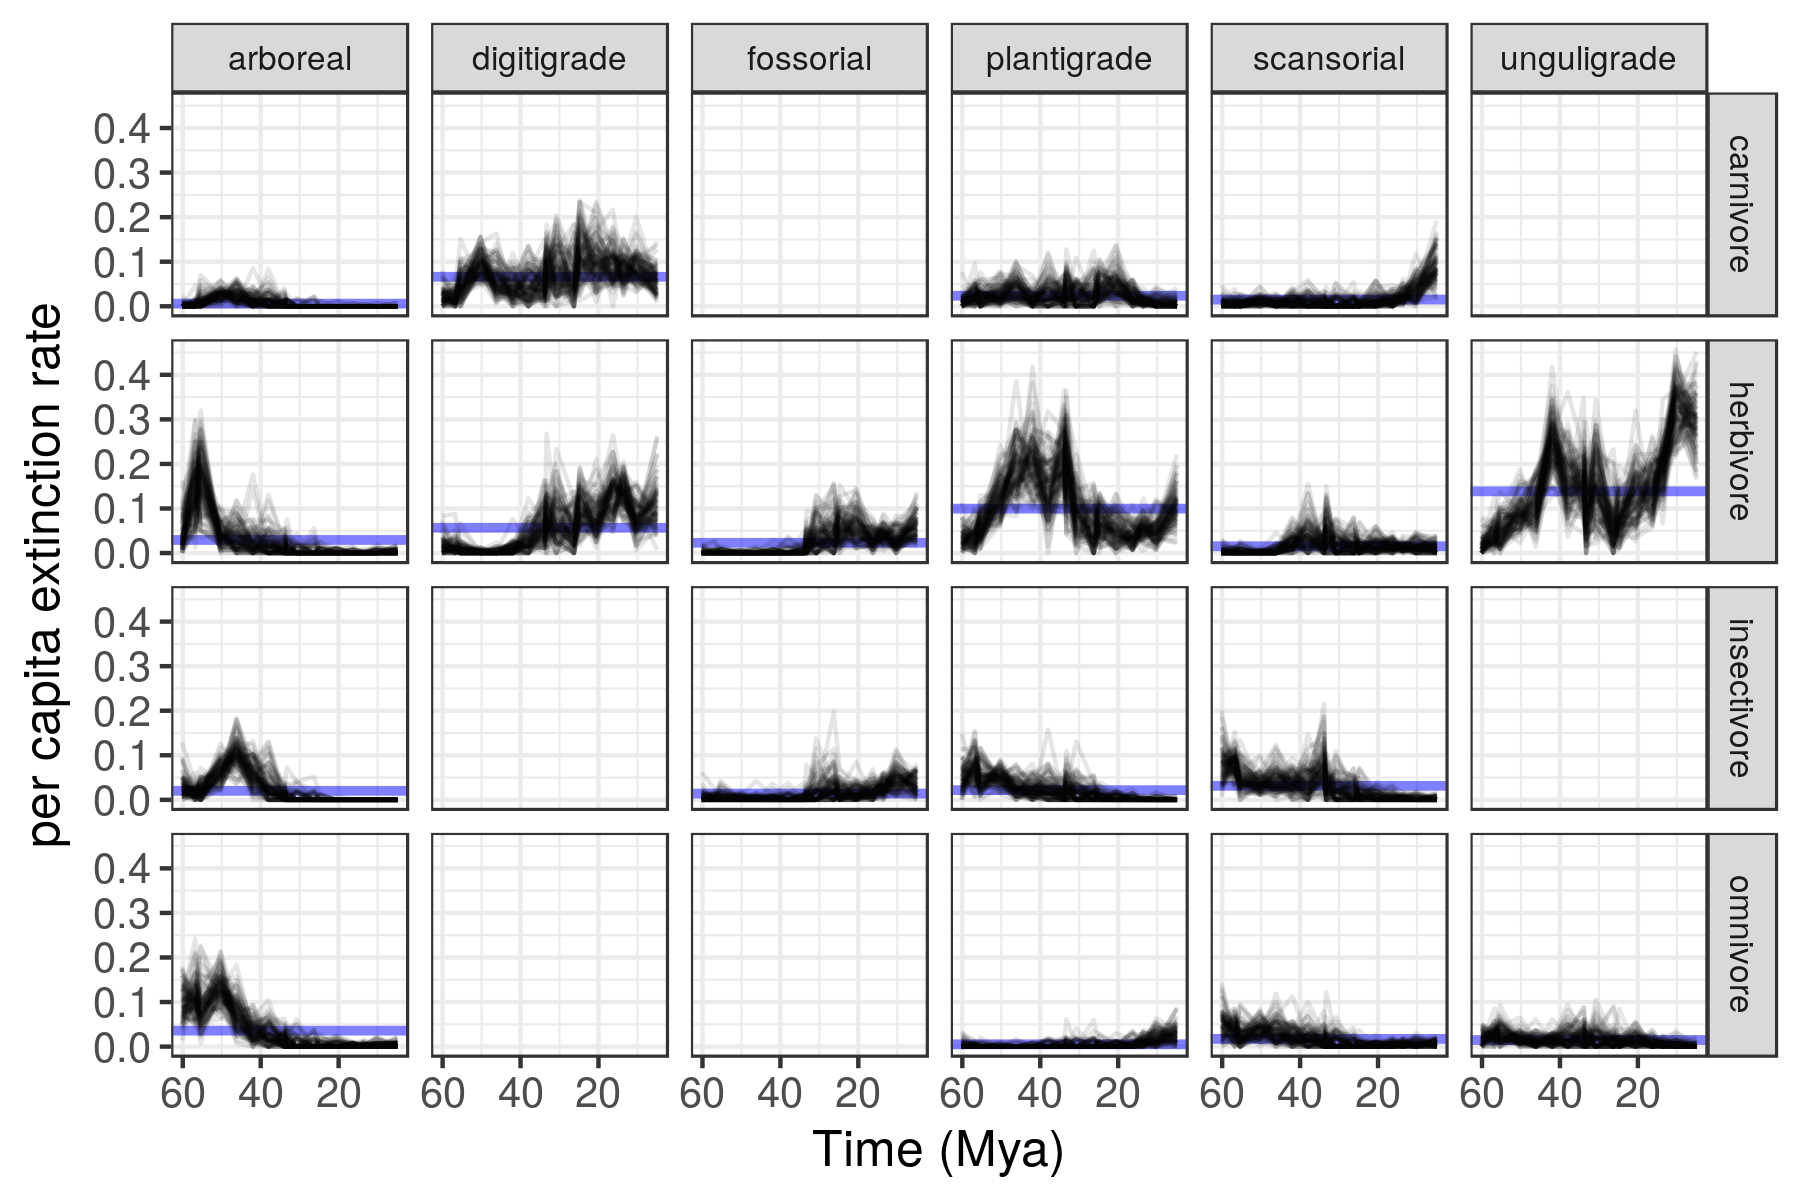
\includegraphics[width=\textwidth,height=0.4\textheight,keepaspectratio=true]{figure/death_eco}
  \caption[Estimated number of extinction events by mammal ecotype]{Posterior estimates of the number of extinction events from one temporal bin to another, plotted at the bin they go extinct from. 100 posterior draws are plotted to indicate the uncertainty in these estimates. Also, what is ploted is log of the number of extinctions plus 1.}
  \label{fig:ecotype_death}
\end{figure}



\end{document}
